% Options for packages loaded elsewhere
% Options for packages loaded elsewhere
\PassOptionsToPackage{unicode}{hyperref}
\PassOptionsToPackage{hyphens}{url}
\PassOptionsToPackage{dvipsnames,svgnames,x11names}{xcolor}
%
\documentclass[
  french,
  12pt,
  letterpaper,
  DIV=11,
  numbers=noendperiod]{scrartcl}
\usepackage{xcolor}
\usepackage[a4paper,left=25mm,right=25mm,top=25mm,bottom=25mm]{geometry}
\usepackage{amsmath,amssymb}
\setcounter{secnumdepth}{-\maxdimen} % remove section numbering
\usepackage{iftex}
\ifPDFTeX
  \usepackage[T1]{fontenc}
  \usepackage[utf8]{inputenc}
  \usepackage{textcomp} % provide euro and other symbols
\else % if luatex or xetex
  \usepackage{unicode-math} % this also loads fontspec
  \defaultfontfeatures{Scale=MatchLowercase}
  \defaultfontfeatures[\rmfamily]{Ligatures=TeX,Scale=1}
\fi
\usepackage{lmodern}
\ifPDFTeX\else
  % xetex/luatex font selection
\fi
% Use upquote if available, for straight quotes in verbatim environments
\IfFileExists{upquote.sty}{\usepackage{upquote}}{}
\IfFileExists{microtype.sty}{% use microtype if available
  \usepackage[]{microtype}
  \UseMicrotypeSet[protrusion]{basicmath} % disable protrusion for tt fonts
}{}
\makeatletter
\@ifundefined{KOMAClassName}{% if non-KOMA class
  \IfFileExists{parskip.sty}{%
    \usepackage{parskip}
  }{% else
    \setlength{\parindent}{0pt}
    \setlength{\parskip}{6pt plus 2pt minus 1pt}}
}{% if KOMA class
  \KOMAoptions{parskip=half}}
\makeatother
% Make \paragraph and \subparagraph free-standing
\makeatletter
\ifx\paragraph\undefined\else
  \let\oldparagraph\paragraph
  \renewcommand{\paragraph}{
    \@ifstar
      \xxxParagraphStar
      \xxxParagraphNoStar
  }
  \newcommand{\xxxParagraphStar}[1]{\oldparagraph*{#1}\mbox{}}
  \newcommand{\xxxParagraphNoStar}[1]{\oldparagraph{#1}\mbox{}}
\fi
\ifx\subparagraph\undefined\else
  \let\oldsubparagraph\subparagraph
  \renewcommand{\subparagraph}{
    \@ifstar
      \xxxSubParagraphStar
      \xxxSubParagraphNoStar
  }
  \newcommand{\xxxSubParagraphStar}[1]{\oldsubparagraph*{#1}\mbox{}}
  \newcommand{\xxxSubParagraphNoStar}[1]{\oldsubparagraph{#1}\mbox{}}
\fi
\makeatother


\usepackage{longtable,booktabs,array}
\usepackage{calc} % for calculating minipage widths
% Correct order of tables after \paragraph or \subparagraph
\usepackage{etoolbox}
\makeatletter
\patchcmd\longtable{\par}{\if@noskipsec\mbox{}\fi\par}{}{}
\makeatother
% Allow footnotes in longtable head/foot
\IfFileExists{footnotehyper.sty}{\usepackage{footnotehyper}}{\usepackage{footnote}}
\makesavenoteenv{longtable}
\usepackage{graphicx}
\makeatletter
\newsavebox\pandoc@box
\newcommand*\pandocbounded[1]{% scales image to fit in text height/width
  \sbox\pandoc@box{#1}%
  \Gscale@div\@tempa{\textheight}{\dimexpr\ht\pandoc@box+\dp\pandoc@box\relax}%
  \Gscale@div\@tempb{\linewidth}{\wd\pandoc@box}%
  \ifdim\@tempb\p@<\@tempa\p@\let\@tempa\@tempb\fi% select the smaller of both
  \ifdim\@tempa\p@<\p@\scalebox{\@tempa}{\usebox\pandoc@box}%
  \else\usebox{\pandoc@box}%
  \fi%
}
% Set default figure placement to htbp
\def\fps@figure{htbp}
\makeatother



\ifLuaTeX
\usepackage[bidi=basic]{babel}
\else
\usepackage[bidi=default]{babel}
\fi
% get rid of language-specific shorthands (see #6817):
\let\LanguageShortHands\languageshorthands
\def\languageshorthands#1{}


\setlength{\emergencystretch}{3em} % prevent overfull lines

\providecommand{\tightlist}{%
  \setlength{\itemsep}{0pt}\setlength{\parskip}{0pt}}



 


% =============================================================
%  HEADER — Dossier_Final_groupe17 |  ENSAI 2026-2027
%  Projet : Laborscope
%  Les "chapitres" sont des \section redéfinies visuellement.
% =============================================================

% ---------- Langue ----------
%\usepackage[french]{babel}
\addto\captionsfrench{%
  \renewcommand{\listfigurename}{Liste des figures}%
  \renewcommand{\listtablename}{Liste des tableaux}%
  \renewcommand{\contentsname}{Table des matières}%
  \renewcommand{\figurename}{Figure}%
  \renewcommand{\tablename}{Tableau}%
}
\AtBeginDocument{%
  \renewcommand{\listfigurename}{Liste des figures}%
  \renewcommand{\listtablename}{Liste des tableaux}%
  \renewcommand{\contentsname}{Table des matières}%
  \renewcommand{\figurename}{Figure}%
  \renewcommand{\tablename}{Tableau}%
  \hypersetup{linkcolor=black}%
}

% ---------- Polices ----------
\usepackage{fontspec}
\usepackage{unicode-math}
%\usepackage{lmodern}
%\setmainfont{Source Sans Pro}

% ---------- Interligne ----------
\usepackage{setspace}
\onehalfspacing


% ---------- Maths ----------
\usepackage{amsmath}
\usepackage{amssymb}
\everymath{\displaystyle}

% ---------- Graphiques & tableaux ----------
\usepackage{graphicx}
\usepackage{float}
\usepackage{array}
\usepackage{booktabs}
\usepackage{multirow}
\usepackage{longtable}
\usepackage{threeparttable}
\renewcommand{\arraystretch}{1.5}
\setlength{\textfloatsep}{8pt}
\setlength{\intextsep}{8pt}

% ---------- PDF ----------
\usepackage{pdfpages}

% =============================================================
%  PALETTE
% =============================================================
\usepackage{xcolor}
\definecolor{MainColor}{HTML}{1565C0}      % bleu principal
\definecolor{AccentColor}{HTML}{7B2FBE}    % violet du cadre titre
\definecolor{MainLight}{HTML}{E0F4FF}      % bleu très clair fond
\definecolor{NeutralColor}{HTML}{546E7A}   % gris-bleu neutre
\definecolor{AccentLight}{HTML}{F3E8FF}    % violet très clair
\definecolor{PurpleColor}{HTML}{FF6F00}    % orange accent
\definecolor{PurpleLight}{HTML}{FFF3E0}    % orange très clair
\definecolor{bg}{rgb}{0.96,0.96,0.96}

% ---------- Tableaux ----------
\usepackage{colortbl}
\arrayrulecolor{white}

% ---------- Minted (un seul chargement) ----------
\usepackage{minted}
\makeatletter\let\listoflistings\@undefined\makeatother
\usemintedstyle{friendly}
\setminted{
  bgcolor=bg, fontsize=\small, linenos=true,
  numbersep=6pt, framesep=2mm, breaklines=true, baselinestretch=1.1
}
\renewcommand{\theFancyVerbLine}{%
  \textcolor{NeutralColor}{\small\arabic{FancyVerbLine}}%
}

% ---------- Hyperref ----------
\usepackage[colorlinks=true, linkcolor=black,
            urlcolor=AccentColor, citecolor=MainColor]{hyperref}
\usepackage[french]{cleveref}

% ---------- Mise en page ----------
\usepackage{geometry}
\geometry{a4paper, left=25mm, right=25mm, top=25mm, bottom=25mm}

% ---------- TikZ & tcolorbox ----------
\usepackage{tikz}
\usetikzlibrary{shapes.geometric}
\usepackage[most]{tcolorbox}

\tcbset{
  isebase/.style={
    coltitle=white, fonttitle=\bfseries\small,
    arc=3pt, boxrule=0pt,
    left=8pt, right=8pt, top=5pt, bottom=5pt, titlerule=0pt,
    attach boxed title to top left={yshift=-2mm, xshift=6pt},
    boxed title style={arc=2pt, boxrule=0pt, left=4pt, right=4pt},
    breakable
  }
}

\newtcolorbox{definition}[1][]{isebase,enhanced,
  title={Définition}, colback=MainLight, colframe=MainColor,
  colbacktitle=MainColor, frame hidden,
  borderline west={3pt}{0pt}{MainColor}, #1}

\newtcolorbox{theoreme}[1][]{isebase,enhanced,
  title={Théorème}, colback=MainLight, colframe=MainColor,
  colbacktitle=MainColor, frame hidden,
  borderline west={3pt}{0pt}{MainColor}, #1}

\newtcolorbox{modele}[1][]{isebase,enhanced,
  title={Modèle}, colback=MainLight, colframe=MainColor,
  colbacktitle=MainColor, frame hidden,
  borderline west={3pt}{0pt}{MainColor}, #1}

\newtcolorbox{hypotheses}[1][]{isebase,enhanced,
  title={Hypothèses}, colback=MainLight, colframe=MainColor,
  colbacktitle=MainColor, frame hidden,
  borderline west={3pt}{0pt}{MainColor}, #1}

% decision = même style que hypotheses
\newtcolorbox{decision}[1][]{isebase,enhanced,
  title={Règle de décision}, colback=MainLight, colframe=MainColor,
  colbacktitle=MainColor, frame hidden,
  borderline west={3pt}{0pt}{MainColor}, #1}

\newtcolorbox{remarque}[1][]{isebase,enhanced,
  title={Remarque}, colback=AccentLight, colframe=AccentColor,
  colbacktitle=AccentColor, frame hidden,
  borderline west={3pt}{0pt}{AccentColor}, #1}

\newtcolorbox{attention}[1][]{isebase,enhanced,
  title={Attention}, colback=AccentLight, colframe=AccentColor,
  colbacktitle=AccentColor, frame hidden,
  borderline west={4pt}{0pt}{AccentColor}, #1}

\newtcolorbox{resultat}[1][]{isebase,enhanced,
  title={Résultat}, colback=PurpleLight, colframe=PurpleColor,
  colbacktitle=PurpleColor, frame hidden,
  borderline west={3pt}{0pt}{PurpleColor}, #1}

% ---------- En-têtes & pieds ----------
\usepackage{fancyhdr}
\pagestyle{fancy}
\fancyhf{}
\renewcommand{\headrulewidth}{0pt}
\renewcommand{\footrulewidth}{0pt}
%\renewcommand{\headrule}{%
%  \vspace{-4pt}{\color{MainColor}\rule{\headwidth}{1.5pt}}}

\fancyhead[L]{}
\fancyhead[R]{}
\fancyfoot[C]{%
  \begin{tikzpicture}[baseline=-0.5ex]
    \node[circle, draw=MainColor, fill=white, text=MainColor,
          inner sep=2pt, font=\small\bfseries, line width=0.8pt]{\thepage};
  \end{tikzpicture}}
\fancyfoot[L]{}
\fancyfoot[R]{\small\color{NeutralColor}\textcopyright\ ENSAI 2026-2027}

\fancypagestyle{plain}{%
  \fancyhf{}
  \renewcommand{\headrulewidth}{0pt}
  \renewcommand{\footrulewidth}{0pt}
  \fancyfoot[L]{%
    \begin{tikzpicture}[baseline=-0.5ex]
      \node[circle, draw=MainColor, fill=white, text=MainColor,
            inner sep=2pt, font=\small\bfseries, line width=0.8pt]{\thepage};
    \end{tikzpicture}}
  \fancyfoot[C]{\small\color{NeutralColor}\textcopyright\ ENSAI 2026-2027}
}

% =============================================================
%  FORMATAGE DES TITRES — titlesec + compteurs indépendants
%  Rapport : Projet Laborscope-Groupe 17
%
%  CAUSE DU BUG "1.0.0" :
%  \titleformat{\section}[block] passe le titre à \sectiontitre
%  AVANT d'incrémenter \arabic{section}. Donc \thesection affiche
%  \chapnum.0 au lieu de \chapnum.1 pour la première section.
%
%  SOLUTION : on n'utilise pas \arabic{section} du tout.
%  On crée des compteurs indépendants (isesecnum, isesubsecnum)
%  qu'on incrémente NOUS-MÊMES au début de \sectiontitre /
%  \subsectiontitre — après le rendu réel de \mychapter.
%
%  SUPPRESSION DES DOUBLONS TDC :
%  scrartcl ajoute automatiquement des entrées TDC pour chaque
%  \section/\subsection/\subsubsection. Nos commandes ajoutent
%  déjà les entrées manuellement via \addcontentsline.
%  On désactive les entrées automatiques en mettant tocdepth à -2.
%
%  STRUCTURE DU RAPPORT :
%  Introduction → Chapitre 1 (cahier de charges) →
%  Chapitre 2 (Modélisation de l'application) → Chapitre 3 (Implémentation) → 
%Chapitre 4 (Fonctionnement de l'application)
%Chapitre 5(Retour sur le projet)  Conclusion
% =============================================================
\usepackage{titlesec}

% Désactiver les entrées TDC automatiques de scrartcl
% (nos \addcontentsline manuels dans \sectiontitre etc. suffisent)
\setcounter{tocdepth}{-2}
\setcounter{secnumdepth}{-2}

% ── Compteur chapitre ─────────────────────────────────────────
\newcounter{chapnum}
\renewcommand{\thechapnum}{\arabic{chapnum}}

% ── Compteurs sections (remis à 0 par \mychapter / \sectiontitre)
\newcounter{isesecnum}
\renewcommand{\theisesecnum}{\thechapnum.\arabic{isesecnum}}

\newcounter{isesubsecnum}
\renewcommand{\theisesubsecnum}{\theisesecnum.\arabic{isesubsecnum}}

\newcounter{isesubsubsecnum}
\renewcommand{\theisesubsubsecnum}{\theisesubsecnum.\arabic{isesubsubsecnum}}

% ── \mychapter : badge numéroté ───────────────────────────────
\newcommand{\mychapter}[1]{%
  \refstepcounter{chapnum}%
  \setcounter{isesecnum}{0}%
  \setcounter{isesubsecnum}{0}%
  \setcounter{isesubsubsecnum}{0}%
  \addcontentsline{toc}{chapter}{\protect\numberline{\thechapnum}#1}%
  \vspace{30pt}%
  \noindent
  \begin{tikzpicture}
    \node[text=MainColor, font=\small\itshape, anchor=south west]
      at (0,4.0em) {Chapitre};
    \node[fill=MainColor, text=white,
          font=\fontsize{48}{48}\selectfont\bfseries,
          minimum width=1.6em, minimum height=1.6em,
          inner sep=6pt, anchor=south west] (nb) at (0,0) {\thechapnum};
    \node[text=MainColor, font=\Large\bfseries,
          anchor=south west, text width=0.72\textwidth, align=left]
      at ([xshift=12pt] nb.south east) {\MakeUppercase{#1}};
  \end{tikzpicture}%
  \vspace{6pt}\par
}

% ── \mychapterstar : chapitre non numéroté ────────────────────
\newcommand{\mychapterstar}[1]{%
  \addcontentsline{toc}{chapter}{#1}%
  \vspace{4pt}%
  \noindent{\Large\bfseries\color{MainColor}\MakeUppercase{#1}}\par
  \vspace{4pt}\par%
}

% ── Sections (## dans Quarto → \subsection dans scrartcl) ────
% Dans scrartcl : # → \section, ## → \subsection, ### → \subsubsection
% Nos "chapitres" sont gérés manuellement via \mychapter.
% Donc ## correspond visuellement à nos sections numérotées.
\newcommand{\sectiontitre}[1]{%
  \refstepcounter{isesecnum}%
  \setcounter{isesubsecnum}{0}%
  \setcounter{isesubsubsecnum}{0}%
  \addcontentsline{toc}{section}{\theisesecnum\quad #1}%
  \noindent
  \begin{tikzpicture}
    \node[fill=MainColor, text=white, font=\bfseries\normalsize,
          inner sep=5pt, minimum width=2.4em, minimum height=1.6em,
          anchor=base west] (sn) at (0,0) {\theisesecnum};
    \node[text=MainColor, font=\bfseries\normalsize, anchor=base west]
      at ([xshift=8pt] sn.base east) {\MakeUppercase{#1}};
  \end{tikzpicture}%
  \vspace{-2pt}{\color{MainColor}\hrule height 0.8pt}\vspace{2pt}%
}
\titleformat{\subsection}[block]{}{}{0pt}{\sectiontitre}
\titlespacing*{\subsection}{0pt}{14pt}{2pt}

% ── Sous-sections (### dans Quarto → \subsubsection dans scrartcl) ────
\newcommand{\subsectiontitre}[1]{%
  \refstepcounter{isesubsecnum}%
  \setcounter{isesubsubsecnum}{0}%
  \addcontentsline{toc}{subsection}{\theisesubsecnum\quad #1}%
  \noindent
  \begin{tikzpicture}
    \node[fill=MainColor, text=white, font=\bfseries\small,
          inner sep=4pt, minimum width=3em, minimum height=1.4em,
          anchor=base west] (ss) at (0,0) {\theisesubsecnum};
    \node[text=MainColor, font=\bfseries\small, anchor=base west]
      at ([xshift=6pt] ss.base east) {#1};
  \end{tikzpicture}%
  \vspace{-2pt}{\color{MainColor!40}\hrule height 0.6pt}\vspace{2pt}%
}
\titleformat{\subsubsection}[block]{}{}{0pt}{\subsectiontitre}
\titlespacing*{\subsubsection}{0pt}{5pt}{2pt}

% ── Sous-sous-sections (#### dans Quarto → \paragraph dans scrartcl) ──
\newcommand{\subsubsectiontitre}[1]{%
  \refstepcounter{isesubsubsecnum}%
  \noindent{\normalsize\itshape\color{NeutralColor}\theisesubsubsecnum\enspace #1}%
}
\titleformat{\paragraph}[block]{}{}{0pt}{\subsubsectiontitre}
\titlespacing*{\paragraph}{0pt}{6pt}{2pt}

% -------------------------------------------------------
% Entrées TDM pour le niveau "chapter" manuel
% -------------------------------------------------------
%  TDM — chapter/section/subsection tous en mode manuel
%  (les entrées viennent de \addcontentsline dans les
%   commandes \mychapter, \sectiontitre, \subsectiontitre)
% -------------------------------------------------------
\usepackage{tocloft}

\renewcommand{\cfttoctitlefont}{\Huge\bfseries\color{black}}
\renewcommand{\cftloftitlefont}{\Huge\bfseries\color{black}}
\renewcommand{\cftlottitlefont}{\Huge\bfseries\color{black}}
\renewcommand{\cftdotsep}{3}

\makeatletter
% Style pour les chapitres (ajoutés via \addcontentsline{toc}{chapter})
\def\l@chapter#1#2{%
  \addpenalty{-\@highpenalty}%
  \vskip 8pt \@plus\p@
  \begingroup
    \parindent\z@ \rightskip\@pnumwidth
    \parfillskip-\@pnumwidth
    {\bfseries\color{black} #1}\nobreak\hfill\nobreak
    \hb@xt@\@pnumwidth{\hss\bfseries\color{black}#2}\par
    \penalty\@highpenalty
  \endgroup
}
% Style pour les sections (ajoutées via \addcontentsline{toc}{section})
\def\l@section#1#2{%
  \vskip 3pt
  \begingroup
    \parindent\z@ \rightskip\@pnumwidth
    \parfillskip-\@pnumwidth
    \hspace{1.5em}{\color{black} #1}\nobreak\dotfill\nobreak
    \hb@xt@\@pnumwidth{\hss\color{black}#2}\par
  \endgroup
}
% Style pour les sous-sections (ajoutées via \addcontentsline{toc}{subsection})
\def\l@subsection#1#2{%
  \vskip 2pt
  \begingroup
    \parindent\z@ \rightskip\@pnumwidth
    \parfillskip-\@pnumwidth
    \hspace{3em}{\small\color{black} #1}\nobreak\dotfill\nobreak
    \hb@xt@\@pnumwidth{\hss\small\color{black}#2}\par
  \endgroup
}
\makeatother

% ---------- Listes ----------
\usepackage{enumitem,pifont}
\setlist[itemize,1]{label={\color{AccentColor}\textbullet}}
\setlist[itemize,2]{label={\color{MainColor}$\circ$}}

\AtBeginDocument{
  \floatplacement{table}{H}
  \floatplacement{figure}{H}
}
\usepackage{booktabs}
\usepackage{longtable}
\usepackage{array}
\usepackage{multirow}
\usepackage{wrapfig}
\usepackage{float}
\usepackage{colortbl}
\usepackage{pdflscape}
\usepackage{tabu}
\usepackage{threeparttable}
\usepackage{threeparttablex}
\usepackage[normalem]{ulem}
\usepackage{makecell}
\usepackage{xcolor}
\KOMAoption{captions}{tableheading}
\makeatletter
\@ifpackageloaded{caption}{}{\usepackage{caption}}
\AtBeginDocument{%
\ifdefined\contentsname
  \renewcommand*\contentsname{Table des matières}
\else
  \newcommand\contentsname{Table des matières}
\fi
\ifdefined\listfigurename
  \renewcommand*\listfigurename{Liste des Figures}
\else
  \newcommand\listfigurename{Liste des Figures}
\fi
\ifdefined\listtablename
  \renewcommand*\listtablename{Liste des Tables}
\else
  \newcommand\listtablename{Liste des Tables}
\fi
\ifdefined\figurename
  \renewcommand*\figurename{Figure}
\else
  \newcommand\figurename{Figure}
\fi
\ifdefined\tablename
  \renewcommand*\tablename{Table}
\else
  \newcommand\tablename{Table}
\fi
}
\@ifpackageloaded{float}{}{\usepackage{float}}
\floatstyle{ruled}
\@ifundefined{c@chapter}{\newfloat{codelisting}{h}{lop}}{\newfloat{codelisting}{h}{lop}[chapter]}
\floatname{codelisting}{Listing}
\newcommand*\listoflistings{\listof{codelisting}{Liste des Listings}}
\makeatother
\makeatletter
\makeatother
\makeatletter
\@ifpackageloaded{caption}{}{\usepackage{caption}}
\@ifpackageloaded{subcaption}{}{\usepackage{subcaption}}
\makeatother
\usepackage{bookmark}
\IfFileExists{xurl.sty}{\usepackage{xurl}}{} % add URL line breaks if available
\urlstyle{same}
\hypersetup{
  pdflang={fr},
  colorlinks=true,
  linkcolor={blue},
  filecolor={Maroon},
  citecolor={Blue},
  urlcolor={Blue},
  pdfcreator={LaTeX via pandoc}}


\author{}
\date{}
\begin{document}


\tableofcontents
\newpage
\listoftables
\newpage
\listoffigures
\newpage

\mychapterstar{REMERCIEMENTS}

Nous tenons à exprimer notre sincère gratitude à toutes les personnes
qui ont contribué, de près ou de loin, à la réalisation de ce projet.

Nos remerciements vont tout d'abord à \textbf{M. Ludovic DENEUVILLE},
responsable du module, pour son encadrement.

Nous remercions tout particulièrement \textbf{M. Anas KNEFATI}, notre
tuteur, pour sa disponibilité, la pertinence de ses conseils et ses
remarques constructives, qui nous ont permis de faire progresser le
projet à chaque étape.

Nous adressons également nos remerciements à l'ensemble de l'équipe
pédagogique de l'École nationale de la statistique et de l'analyse de
l'information (ENSAI) pour la qualité de la formation dispensée et les
ressources mises à notre disposition.

Enfin, nous félicitons les membres du groupe pour leur investissement,
leur esprit d'équipe et leur bonne humeur durant ces mois de travail.
\newpage

\mychapterstar{Résumé} 

Le projet \textbf{LaborScope} vise à rendre accessible l'exploration des
données du marché du travail mondial, issues de la base ILOSTAT de
l'Organisation internationale du Travail (OIT). Cette base, très riche,
rassemble de nombreux indicateurs (emploi, chômage, secteurs d'activité,
inégalités entre les sexes\ldots), mais sa taille et sa complexité en
limitent l'usage par des utilisateurs non spécialistes.

Pour répondre à ce besoin, nous avons conçu et développé une application
interactive permettant de {[}sélectionner un pays, une période et un
indicateur{]}, de {[}visualiser les évolutions sous forme de graphiques
et de cartes{]} et de {[}comparer plusieurs pays ou régions{]}. La
démarche suivie comprend une étude préalable (cahier des charges,
identification des utilisateurs, structure de la base de données), une
phase de conception fondée sur des diagrammes UML (cas d'utilisation,
classes, activités, séquences), puis une phase de réalisation reposant
sur {[}Python, une base de données relationnelle et une interface
web{]}.

L'application obtenue permet {[}d'explorer rapidement les données
ILOSTAT et d'en dégager des tendances{]}, tout en gérant les difficultés
propres à ces données : valeurs manquantes, couverture inégale selon les
pays et les années, hétérogénéité des définitions. Ce rapport présente
la conception, la réalisation et les résultats du projet, puis en dresse
les limites et les perspectives d'évolution.

\textbf{Mots-clés :} marché du travail, ILOSTAT, visualisation de
données, application interactive, conception UML

\newpage

\mychapterstar{INTRODUCTION}

Le marché du travail est au cœur des préoccupations économiques et
sociales contemporaines. Chômage, emploi informel, inégalités entre les
sexes ou encore évolution des secteurs d'activité : ces indicateurs
conditionnent les politiques publiques et les décisions des
organisations internationales, des entreprises et des chercheurs.
L'Organisation internationale du Travail (OIT) en assure le suivi à
l'échelle mondiale grâce à sa base de données ILOSTAT, qui rassemble des
milliers d'indicateurs harmonisés couvrant la plupart des pays du monde.

Cette richesse constitue pourtant une difficulté. Le volume et la
diversité des données rendent leur exploration fastidieuse pour un
utilisateur non spécialiste : il faut identifier les bons indicateurs,
comprendre leurs définitions, gérer les valeurs manquantes et les
différences de couverture entre pays et entre années, puis produire des
comparaisons lisibles. Il manque ainsi un outil simple, accessible et
interactif permettant d'explorer ces données et d'en dégager rapidement
des enseignements.

C'est dans ce contexte que s'inscrit le projet \textbf{LaborScope},
réalisé dans le cadre de notre formation à l'École nationale de la
statistique et de l'analyse de l'information (ENSAI). Son objectif est
de concevoir et de développer une application d'analyse interactive du
marché du travail mondial à partir des données ILOSTAT. Elle doit
permettre à l'utilisateur de {[}sélectionner un pays, une période et un
indicateur{]}, de {[}visualiser les évolutions sous forme de graphiques
et de cartes{]} et de {[}comparer plusieurs pays ou régions{]}, le tout
au sein d'une interface claire et ergonomique.

Dans le rapport intermédiaire, nous avons posé les bases du projet :
cahier des charges, identification des utilisateurs, fonctionnalités
attendues, structure de la base de données et organisation du travail en
équipe. Le présent rapport final en constitue l'aboutissement. Il
présente la conception détaillée de l'application, sa réalisation, les
choix techniques effectués ainsi que les résultats obtenus.

Ce document s'organise en cinq (05) chapitres. Le premier rappelle
l'étude préalable (contexte, cahier des charges et architecture
générale). Le deuxième expose le modèle de conception à travers les
diagrammes UML (cas d'utilisation, classes, activités et séquences). Le
troisième décrit la réalisation de l'application : technologies
employées, implémentation des fonctionnalités et analyse des résultats.
Le quatrième chapitre explique en détail les différentes fonctionnalités
présentes dans l'application.Enfin, le dernier chapitre évoque les
retours de chaque membre du groupe par rapport au projet.

\newpage

\mychapter{Description du projet}

\sectiontitre{Le cahier de charges}

\subsectiontitre{Présentation d’ensemble du projet}

Le ``LaborScope'' est une application dédiée à l'analyse des
statistiques mondiales du marché du travail. C'est une application
interactive alimentée par les données ouvertes de l'Organisation
Internationale du Travail (ILOSTAT). L'objectif de cette application est
dans un premier temps, de récupérer des données brutes (des indicateurs)
comme l'emploi par sexe et profession, ou la population en âge de
travailler depuis le site, de les extraire et de les stocker localement
pour des fins d'analyse et de visualisation.

C'est une application sécurisée (avec gestion des utilisateurs et
administrateurs) disposant de différentes fonctionnalités permettant de
suivre l'évolution des indicateurs dans le temps, faire une comparaison
entre plusieurs pays ou croiser plusieurs indicateurs sur un même
graphique. Elle peut être complétée par une interface web interactive
(Streamlit) pour visualiser les résultats sans avoir à coder et générer
automatiquement un rapport d'analyse au format PDF.

L'objectif final est de transformer des données statistiques brutes et
complexes en un outil simple qui permet de comprendre, comment évolue
l'emploi dans le monde et comment les pays se comparent entre eux.

\subsectiontitre{Identification des utilisateurs}

On distingue deux types de profils dans l'accès aux fonctionnalités de
l'application: les utilisateurs et les administrateurs.

Les utilisateurs disposent d'un compte classique leur permettant de
consulter des analyses, et de visualiser les données. Ils peuvent
également générer de manière automatique des rapports d'analyse au
format PDF contenant les données qu'ils ont consultées. Les
administrateurs sont chargés de la gestion des comptes utilisateurs
classiques et peuvent modifier ou supprimer des données. Ils peuvent
également faire un suivi des activités. Les utilisateurs de
l'application ne peuvent pas obtenir le statut d'administrateur. Ceci
permet de mieux contrôler l'accès aux modifications des données.

\sectiontitre{Méthodologie de travail et organisation de l'équipe}

\subsectiontitre{Méthode de travail}

Pour livrer notre application à temps, nous avons réalisé un diagramme
de GANTT. C'est un calendrier prévisionnel avec les différentes tâches à
réaliser et leur durée estimée. Ce type de diagramme est indispensable
pour avoir une bonne vision de l'avancement du projet et ne pas perdre
de vue les dates de rendus. \newline Dans le cadre de notre projet, nous
pouvons distinguer cinq grandes étapes :\newline • « Diagramme UML » :
il s'agit ici de modéliser l'ensemble du projet en respectant le cahier
des charges que nous avons établi. Il y a pour cela deux phases. La
première est la phase d'étude. Elle permet de construire le diagramme de
cas d'utilisation. Vient ensuite la phase de conception. Il s'agit alors
de créer les diagrammes d'activités correspondant aux cas d'utilisation
du premier diagramme, le diagramme de classes et celui de la base de
données. Cette étape est cruciale car sans elle, l'implémentation ne
pourra être faite correctement.\newline • « Dossier d'analyse » : pour
s'assurer du bon démarrage du projet, nous avons réalisé un dossier
d'analyse qui regroupe l'ensemble de la planification et de la
modélisation. Chacun d'entre nous ayant participé à la rédaction de ce
rapport, il était important de consacrer du temps à sa conception. Cela
permet d'assurer la cohérence du contenu et d'en faire des
relectures.\newline • « Implémentation » : c'est le temps de la
réalisation du projet. Cette étape comporte l'importation des données à
partir de l'ILOSTAT,la création de la base de données, le développement
de la DAO et la mise en place des différentes fonctionnalités du projet.
C'est la partie la plus longue du projet. Nous avions prévu d'y
consacrer environ 1 mois après le dépot du rapport intermédiaire, or
nous avons eu besoin de 10 jours supplémentaires pour que tout
fonctionne correctement.\newline • « Rapport et code » : Afin de gagner
du temps, nous voulions rédiger le rapport parallèlement à l'étape
d'implémentaion. Cette dernière plus complexe et chronophage que prévu,
nous avons décidé de, finalement, repousser l'écriture au\ldots. Tout
comme pour le dossier d'analyse, nous avons accordé deux jours à la
relecture. Le code final étant à rendre pour le 25 novembre, nous
consacrerons la dernière semaine au dossier final.\newline • «
Soutenance » : pour finir, nous aurons une semaine pour créer un
diaporama afin de présenter notre projet le 09 décembre devant un jury
composé d'un professionnel de l'informatique, de notre encadrant et d'un
représentant de l'ENSAI.\newline

(diagramme de GANTT)

\subsectiontitre{Organisation de l'équipe}

Le projet a été réalisé par cinq membres. Pour avancer en parallèle sans
se bloquer, le travail a été découpé en cinq rôles, chacun décrit dans
une fiche de tâches détaillée (objectifs, fichiers à écrire, étapes,
tutoriels) rédigée par Laurent Khaouli. Le partage suit un principe
simple : deux membres construisent le socle commun, et les trois autres
codent chacun une fonctionnalité complète, de la base de données jusqu'à
l'écran. Cela leur permet de toucher toutes les couches de
l'application.

\textbf{•Le socle commun}

-Clarence Chemla-Vidaud (rôle A : données et administration). Elle est
responsable de tout ce qui touche aux données : import depuis ILOSTAT
(fetcher), base de données, gestion des pays et des modalités, actions
d'administration sur les données (F1, F2 et la partie données de F6).
Elle assure aussi la qualité du projet : infrastructure de tests,
journalisation (logs), intégration continue et README. En fin de projet,
elle a relu l'ensemble du backend, harmonisé le code avec pylint et
simplifié plusieurs fichiers (schémas, controllers).\newline -Laurent
Khaouli (rôle B : utilisateurs, sécurité et squelette frontend). Il gère
les comptes (création, connexion, rôles utilisateur et administrateur,
historique des actions, partie comptes de F6) et construit le squelette
de l'application Streamlit dans lequel chacun a ajouté sa page. Il a
aussi conçu l'organisation du travail en fiches et testé le
fonctionnement des endpoints.

\textbf{•Les fonctionnalités}

-Antifa Badarou (rôle C : évolution d'un indicateur, F3). Elle a codé le
calcul de l'évolution d'un indicateur sur les N derniers trimestres :
service, schéma, controller, tests, puis la page d'affichage des
graphiques. Elle a fournit le template pour la rédaction du dossier
final et effectué des mises en formes et réglages global du
document.Elle a aussi rédigé avec l'aide des autres memebres le dossier
final.\newline

-William Margerand (rôle D : comparaison entre pays, F4, et carte du
monde, FO2). Il a codé le classement des pays pour la période la plus
récente (valeurs les plus hautes et les plus basses) avec ses tests,
puis la carte choroplèthe. Il a ensuite amélioré le choix de la période,
la période commune et les couleurs. Il a rédigé les sections du dossier
consacrées à F4 et FO2, à l'exploration des données, ainsi que le
chapitre 2 de modélisation et le diagramme de cas d'utilisation.\newline

-Christian Adjeba (rôle E : comparaison multi-indicateurs, F5, et
rapport PDF, FO3). Il a codé la comparaison de plusieurs indicateurs sur
un même graphique (schéma, controller, service), puis la génération
automatique du rapport PDF (service, controller, tests et page
frontend). Il a aussi amélioré F5 après les échanges avec le tuteur et
harmonisé les noms d'indicateurs dans le rapport.\newline

\textbf{•Organisation commune}

Chacun a rédigé ses propres sections du dossier final et tenu un compte
rendu hebdomadaire (12 semaines). Les fichiers partagés, comme main.py,
n'ont reçu qu'une ligne par controller, ce qui a limité les conflits.
Les relectures croisées et les échanges réguliers avec le tuteur ont
permis de valider les choix de conception.

\sectiontitre{Réadaptation des diagrammes}

A la suite du dépot du rapport intermédiare,notre tuteur nous a fais des
remarques concernants le diagramme d'architecture et le diagramme de
classe. Nous avons donc intégrer ses remarques et amélioré les
diagrammes concernés.

\subsectiontitre{Diagramme d'architecture}

Voilà ci contre le diagramme d'architecture qui montre la structure
globale de l'API:

\subsectiontitre{Diagramme de classes}

Voila ci après le diagramme de classe corrigé:

\sectiontitre{Normes de codage utilisées}

Pour que n'importe quel programme soit facilement compréhensible par
tous les développeurs informatiques, il existe des conventions de
nommage en python. Ainsi le projet \textbf{Laborscope}, développée en
python suit les règles suivantes :\newline

•Indentation : 4 espaces par niveau (jamais de tabulations mélangées
avec des espaces)\newline •Longueur de ligne : 79 caractères maximum
pour le code (72 pour les commentaires et docstrings). Certaines lignes
s'étendent à 88 ou 100.\newline •Lignes vides : 2 lignes entre les
fonctions et classes de niveau supérieur, 1 ligne entre les
méthodes\newline •Imports : un par ligne, en haut du fichier, regroupés
dans l'ordre : bibliothèque standard, bibliothèques tierces, modules
locaux\newline •Espaces : autour des opérateurs, pas d'espace avant les
parenthèses d'un appel (f(x)), pas d'espace superflu à l'intérieur des
crochets.\newline

Pour faciliter la lecture de notre code, et permettre à d'autres
développeurs de travailler dessus par la suite, nous l'avons commenté.

\newpage

\mychapter{Modelisation de l'application}

Pour bien comprendre l'application \textbf{Laborscope}, nous expliquons
ici l'ensemble des possibilités qu'elle offre selon le type de personne
qui l'utilise, puis la façon de naviguer entre ses différentes pages.
Pour une meilleure conceptualisation, nous nous appuyons sur un
diagramme UML de cas d'utilisation.

\sectiontitre{Diagramme de cas d'utilisation}

L'application distingue trois acteurs :

\begin{itemize}
\tightlist
\item
  le \textbf{visiteur}, qui n'est pas connecté : il peut seulement créer
  un compte ou se connecter ;
\item
  l'\textbf{utilisateur}, connecté avec un compte classique : il a accès
  à toutes les analyses de l'application ;
\item
  l'\textbf{administrateur} : il peut faire tout ce que fait un
  utilisateur (flèche d'héritage sur le diagramme) et dispose en plus
  des fonctions de gestion de l'application.
\end{itemize}

\begin{figure}[H]

{\centering 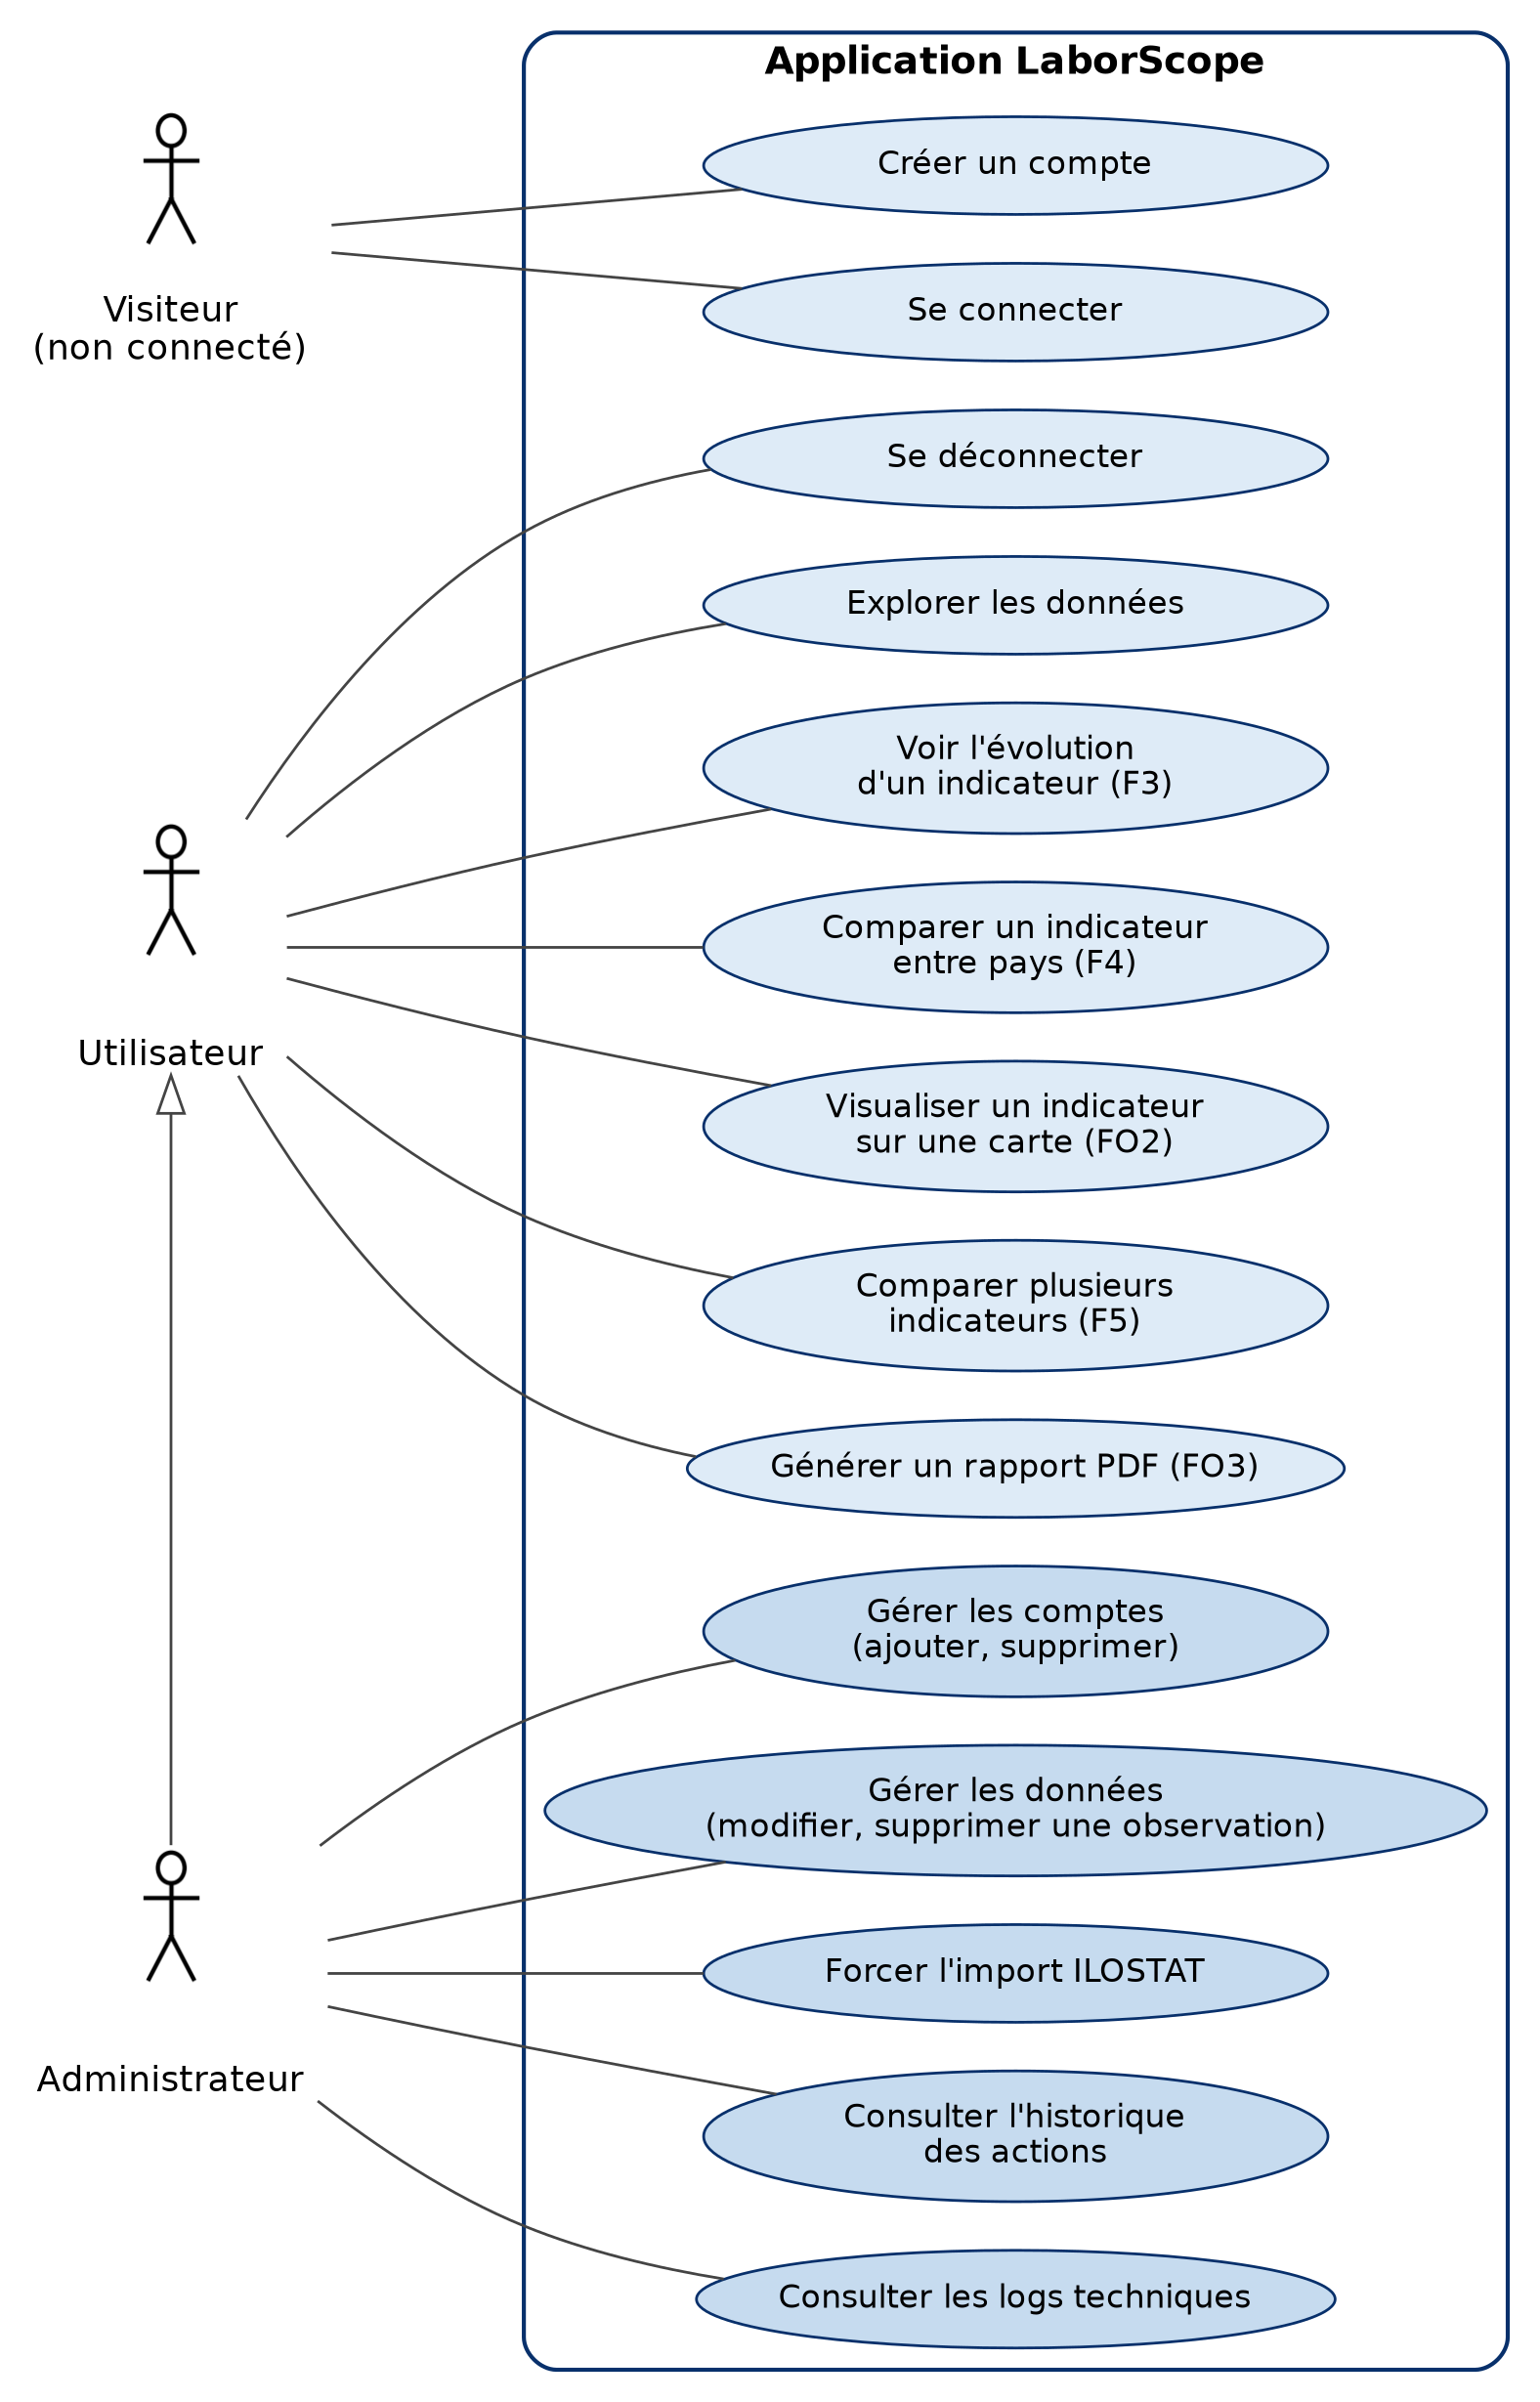
\includegraphics[width=0.42\linewidth,height=\textheight,keepaspectratio]{images/diagramme_cas_utilisation.png}

}

\caption{Diagramme de cas d'utilisation de l'application}

\end{figure}%

Ce diagramme a été mis à jour par rapport à celui du rapport
intermédiaire. Nous y avons ajouté deux cas d'utilisation apparus
pendant le développement : « Explorer les données », qui permet de
consulter les observations brutes de la base, et « Forcer l'import
ILOSTAT », qui permet à un administrateur de recharger toutes les
données depuis l'API de l'OIT.

\sectiontitre{Navigation dans l'application}

L'application se présente sous la forme d'un site web. Un menu latéral,
à gauche de l'écran, permet de passer d'une page à l'autre. Son contenu
change selon le rôle de la personne connectée : chacun ne voit que les
pages auxquelles il a droit.

\subsectiontitre{Accueil et accès au compte}

À l'ouverture de l'application, le visiteur arrive sur la page
d'accueil, qui présente brièvement Laborscope et les données ILOSTAT sur
lesquelles elle s'appuie. Son menu ne contient que trois pages : «
Accueil », « Se connecter » et « Créer un compte ». Deux boutons de la
page d'accueil mènent aussi directement à ces deux dernières pages.

Avant la première connexion, il faut créer un compte à l'aide d'un
pseudo et d'un mot de passe d'au moins 8 caractères, saisi deux fois
pour éviter les fautes de frappe. Deux utilisateurs ne peuvent pas avoir
le même pseudo, ce dernier se doit d'être unique. Une fois le compte
créé, l'utilisateur est connecté automatiquement. Si son compte existe
déjà, il se connecte grâce à son pseudo et son mot de passe.

\subsectiontitre{Menu utilisateur}

Une fois connecté, l'utilisateur retrouve la page d'accueil, qui
l'invite à choisir une analyse dans le menu. Celui-ci contient une
rubrique « Analyses » avec six pages :

\begin{itemize}
\tightlist
\item
  \textbf{Explorer les données} : consulter les observations brutes d'un
  indicateur sous forme de tableau ;
\item
  \textbf{Évolution (F3)} : suivre l'évolution d'un indicateur au cours
  du temps ;
\item
  \textbf{Comparaison pays (F4)} : classer plusieurs pays selon un
  indicateur ;
\item
  \textbf{Carte du monde (FO2)} : afficher un indicateur sur une carte
  du monde ;
\item
  \textbf{Multi-indicateurs (F5)} : comparer plusieurs indicateurs sur
  un même graphique ;
\item
  \textbf{Rapport PDF (FO3)} : générer un rapport synthétique au format
  PDF.
\end{itemize}

Ces pages fonctionnent toutes de la même façon : l'utilisateur choisit
un indicateur, puis les filtres qui l'intéressent (pays, sexe, tranche
d'âge ou profession selon l'indicateur), et le résultat s'affiche sous
forme de tableau, de graphique ou de carte. Elles sont détaillées dans
le chapitre « Fonctionnement de l'application ».

En bas du menu, l'utilisateur voit le pseudo et le rôle avec lesquels il
est connecté, ainsi qu'un bouton « Se déconnecter » qui le ramène au
menu du visiteur.

\subsectiontitre{Menu administrateur}

L'administrateur voit le même menu que l'utilisateur, avec en plus une
rubrique « Administration » composée de trois pages :

\begin{itemize}
\tightlist
\item
  \textbf{Utilisateurs} : afficher la liste des comptes, ajouter un
  compte en choisissant son rôle (utilisateur ou administrateur) et
  supprimer un compte ;
\item
  \textbf{Données} : forcer un nouvel import des données ILOSTAT, et
  modifier ou supprimer manuellement une observation ;
\item
  \textbf{Logs et historique} : consulter, dans deux onglets,
  l'historique des actions (connexions, créations et suppressions de
  comptes, imports et modifications des données\ldots) et les logs
  techniques de l'application.
\end{itemize}

Les actions difficiles à annuler (suppression d'un compte ou d'une
observation, nouvel import qui écrase les modifications manuelles) ne
sont possibles qu'après avoir coché une case de confirmation.

\subsectiontitre{Contrôle des accès}

Cacher les pages dans le menu ne suffit pas à protéger l'application.
Chaque page vérifie donc aussi le rôle de la personne qui l'ouvre : un
visiteur qui accède à une page d'analyse reçoit le message «
Connectez-vous pour accéder à cette page », et un utilisateur qui accède
à une page d'administration reçoit le message « Réservé aux
administrateurs ». Ces droits sont également vérifiés par l'API, qui
refuse les requêtes d'une personne non connectée ou sans les droits
nécessaires. Enfin, si la session n'est plus valable (par exemple après
une réinitialisation de la base de données), l'utilisateur est prévenu
et le menu redevient celui du visiteur.

\newpage

\mychapter{Implémentation}

(obtention des données et fonctionnement du DAO)

Ce chapitre décrit la manière dont LaborScope a été réalisé, depuis les
données brutes d'ILOSTAT jusqu'à l'application interactive utilisée par
l'utilisateur final. Il présente les choix techniques retenus,
l'organisation de la base de donnée et les principaux points de
fonctionnement du DAO.

\sectiontitre{Des données ILOSTAT à la base de données}

\subsectiontitre{Récupération des données}

L'application se base sur les données ouvertes de l'API ILOSTAT. Dans un
premier temps, il nous fallait comprendre comment cette API fonctionne
pour pouvoir décider de la manière d'importer les données.

Le site donne accès à de nombreux indicateurs. Le cahier des charges
nous en imposait deux, et nous en avons choisi trois :

\begin{itemize}
\tightlist
\item
  le taux de chômage par sexe et âge ;
\item
  le taux d'emploi par sexe et âge ;
\item
  l'emploi par sexe et profession.
\end{itemize}

Chaque indicateur a son propre identifiant dans l'URL de l'API (par
exemple \texttt{EMP\_5EMP\_SEX\_OC2\_NB\_Q} pour l'emploi par sexe et
profession). Nous avons choisi de reconstruire chaque URL à partir de
cet identifiant plutôt que de coder les URL en dur. Une URL contient
quatre paramètres : \texttt{id}, le code de l'indicateur ;
\texttt{timefrom}, la première année récupérée ; \texttt{type=both}, qui
permet d'obtenir à la fois le code d'un pays (« FRA ») et son nom («
France ») ; et \texttt{format=.csv}, pour recevoir les données sous
forme de tableau.

Nos différents indicateurs sont stockés dans un fichier :
\texttt{backend/src/config\_import.py}. Ce fichier contient aussi la
liste des 80 pays suivis et l'année de début des données (2020). C'est
le seul fichier à modifier si l'on veut ajouter un indicateur ou un pays
: le reste du code s'adapte automatiquement.

Pour chaque indicateur, l'import fait un appel à l'API par pays. Si un
appel échoue, il est relancé une deuxième fois après 3 secondes. Si ce
deuxième essai échoue aussi, le pays est ignoré et l'import passe au
pays suivant. Ainsi, une erreur sur un pays ne bloque pas toute la
récupération.

\subsectiontitre{Traitement des données}

Le problème est que les tableaux récupérés depuis l'API ne sont pas
propres : certaines colonnes sont superflues et leurs noms ne sont pas
synthétiques. Il nous fallait donc traiter les données après les avoir
récupérées.

Le dossier qui contient tous les fichiers de traitement est
\texttt{src/fetcher/}. Il contient en particulier quatre fichiers :

\begin{itemize}
\tightlist
\item
  \texttt{fetcher.py} : construit les URL nécessaires et télécharge les
  données de l'API sous forme de tableau (DataFrame) ;
\item
  \texttt{parser.py} : nettoie les libellés d'ILOSTAT en retirant leurs
  préfixes ;
\item
  \texttt{data\_processing.py} : utilise les méthodes des deux fichiers
  précédents. Il sélectionne et renomme les colonnes utiles, nettoie les
  tableaux, puis les enregistre dans la base ;
\item
  \texttt{charger\_donnees.py} : script final qui lance l'ensemble :
  récupérer les données d'ILOSTAT, les traiter et les stocker.
\end{itemize}

Le nettoyage, fait par la méthode \texttt{parse\_data} de
\texttt{data\_processing.py}, se déroule en quatre étapes :

\begin{enumerate}
\def\labelenumi{\arabic{enumi}.}
\tightlist
\item
  sélection des colonnes utiles et renommage ;
\item
  conversion des valeurs en nombres, puis suppression des lignes sans
  valeur ;
\item
  nettoyage des libellés : par exemple « Age (Youth, adults): 15-24 »
  devient « 15-24 » et « Sex: Female » devient « Female ». Quand une
  dimension n'existe pas pour un indicateur, on la remplace par
  \texttt{\_NA} ;
\item
  suppression des doublons, c'est-à-dire des lignes qui ont le même
  pays, la même source, la même période, le même sexe et la même
  modalité.
\end{enumerate}

Le tableau suivant montre les colonnes que nous gardons et leur nouveau
nom :

\begin{longtable}[]{@{}lll@{}}
\caption{Colonnes conservées et renommées lors du traitement des
données}\tabularnewline
\toprule\noalign{}
Colonne ILOSTAT & Colonne dans notre base & Exemple \\
\midrule\noalign{}
\endfirsthead
\toprule\noalign{}
Colonne ILOSTAT & Colonne dans notre base & Exemple \\
\midrule\noalign{}
\endhead
\bottomrule\noalign{}
\endlastfoot
\texttt{ref\_area} & \texttt{code\_iso} & FRA \\
\texttt{ref\_area.label} & \texttt{nom\_pays} & France \\
\texttt{time} & \texttt{periode} & 2024Q4 \\
\texttt{sex.label} & \texttt{sexe} & Female \\
\texttt{classif1.label} & \texttt{classif1} & 15-24 \\
\texttt{obs\_value} & \texttt{valeur} & 7,5 \\
\end{longtable}

{[}Graphe simplifié du chemin des données{]}

\subsectiontitre{Stockage, business objects et DAO}

Comme nous ne souhaitions pas stocker chaque tableau dans notre
environnement, nous avons décidé de travailler avec PostgreSQL.
L'objectif est d'avoir nos données sous forme de tables SQL pour pouvoir
les utiliser plus facilement. Les DAO (Data Access Objects) nous
permettent de communiquer avec la base SQL et d'utiliser les données
récupérées.

La structure de la base est définie dans le fichier
\texttt{data/init\_db.sql}, à la racine du projet. Il crée nos trois
tables principales, « indicateur », « pays » et « observation ». Ces
trois tables fonctionnent de manière très simple : « indicateur »
recense tous les indicateurs (3 ici), « pays » recense tous les pays
utilisés, et « observation » contient toutes les lignes des tableaux
provenant d'ILOSTAT, quel que soit l'indicateur. C'est la table la plus
importante de l'application : elle contient toutes les données.

Cette organisation correspond à un modèle en étoile : « observation »
est la table de faits, au centre, et « indicateur » et « pays » sont des
tables de dimensions qui la complètent. Chaque observation fait
référence à un indicateur et à un pays grâce à des clés étrangères. Le
dossier \texttt{data/} contient aussi un second fichier,
\texttt{pop\_db.sql}, qui fournit un petit jeu de données de secours si
l'API est injoignable.

Une observation est identifiée par une clé primaire composée de six
colonnes : l'indicateur, le pays, la source, la période, le sexe et la
modalité. Cette clé nous permet de relancer l'import autant de fois que
nécessaire sans créer de doublons : grâce à la commande SQL
\texttt{INSERT\ ...\ ON\ CONFLICT}, une observation déjà présente n'est
pas ajoutée une deuxième fois, mais sa valeur est mise à jour.

Chacune de ces trois tables a son propre DAO (\texttt{IndicateurDAO},
\texttt{PaysDAO} et \texttt{ObservationDAO}, dans le dossier
\texttt{src/dao/}), qui fait le lien entre PostgreSQL et l'application.
Les DAO sont les seuls fichiers du projet qui contiennent des requêtes
SQL. Ils fonctionnent dans les deux sens :

\begin{itemize}
\tightlist
\item
  en écriture : ils reçoivent un tableau propre et l'insèrent dans la
  base. Les observations sont envoyées par paquets de 1000 lignes pour
  aller plus vite. L'ordre d'enregistrement est important : on
  enregistre d'abord l'indicateur, puis les pays, puis les observations,
  car une observation ne peut pas faire référence à un pays ou à un
  indicateur qui n'existe pas encore ;
\item
  en lecture : ils récupèrent les données pour le reste de
  l'application. Par exemple, la méthode \texttt{lire}
  d'\texttt{ObservationDAO} renvoie les observations d'un indicateur et
  peut les filtrer par pays, période, sexe et modalité.
\end{itemize}

Tous les DAO passent par une seule connexion à la base, gérée par la
classe \texttt{DBConnection}. Elle utilise le patron Singleton : une
seule instance de la classe peut exister, donc une seule connexion est
ouverte et partagée par toute l'application. Les paramètres de connexion
(adresse, nom de la base, identifiants) sont lus dans le fichier
\texttt{.env}, ce qui évite de les écrire dans le code.

Les DAO ne renvoient pas seulement des tableaux : ils peuvent aussi
renvoyer des business objects. Ce sont des classes simples, dans le
dossier \texttt{src/business\_object/}, qui représentent les objets que
manipule l'application :

\begin{itemize}
\tightlist
\item
  \texttt{Indicateur} : le code, le libellé, l'unité, la fréquence et le
  type de modalité d'un indicateur. Ce sont ces objets qui décrivent les
  indicateurs dans \texttt{config\_import.py}. Cette classe vérifie
  aussi ses attributs à la création, par exemple que la fréquence vaut
  bien « Q », « A » ou « M » ;
\item
  \texttt{Pays} : le code ISO et le nom d'un pays, avec des méthodes
  pour retrouver son continent et les groupes auxquels il appartient ;
\item
  \texttt{Selection} : un indicateur et ses filtres (pays, modalité,
  sexe), utilisé pour la comparaison multi-indicateurs.
\end{itemize}

Par exemple, la méthode \texttt{lister} de \texttt{PaysDAO} renvoie une
liste d'objets \texttt{Pays}, et celle d'\texttt{IndicateurDAO} une
liste d'objets \texttt{Indicateur}. Les observations, elles, restent
sous forme de tableaux pandas, car les services font leurs calculs
directement dessus.

{[}Diagramme de classes des business objects{]}

\subsectiontitre{Limites}

Cette chaîne d'import a tout de même quelques limites :

\begin{itemize}
\tightlist
\item
  l'import est lent : comme on fait un appel à l'API par pays et par
  indicateur, il faut plusieurs centaines d'appels pour tout récupérer.
  Ici ce n'est pas encore très contraigant. Si la table ``observation''
  dépasse les 500 milles ligne il faudrait travailler avec d'autres
  outils qui rendent l'import et la lecture plus rapide.
\item
  les données ne remontent qu'à 2020 ;
\item
  la couverture est très inégale selon les pays : certains n'ont qu'un
  seul trimestre dans la base, ce qui limite les comparaisons (voir la
  carte du monde au chapitre 4).
\end{itemize}

\newpage

\mychapter{Fonctionnement de l'application}

(Détails sur les fonctionnalités de l'application)

\sectiontitre{Explorer les données}

\subsectiontitre{Présentation de la fonctionnalité}

La page « Explorer les données » permet de consulter directement les
données ILOSTAT enregistrées dans notre base, sans calcul. L'utilisateur
choisit un indicateur, un ou plusieurs pays, une modalité (une tranche
d'âge ou une profession selon l'indicateur, le total étant proposé par
défaut) et le sexe (Total, Hommes ou Femmes). La page affiche alors un
tableau avec une ligne par observation.

Chaque ligne donne le pays, la période, la valeur et son unité, mais
aussi la source de la donnée (le nom de l'enquête nationale) et son
statut éventuel. Ces informations sont utiles pour savoir d'où vient un
chiffre avant de l'utiliser dans une analyse. Les lignes sont triées par
pays puis par période. Le tableau affiche au plus 100 observations, ce
qui suffit pour quelques pays mais peut couper le résultat si
l'utilisateur en choisit beaucoup.

\subsectiontitre{Fonctionnement technique}

La page repose sur les mêmes couches que le reste de l'application :

\begin{itemize}
\tightlist
\item
  la couche DAO (classe ObservationDAO) construit une requête SQL qui
  joint les tables des observations, des indicateurs et des pays, puis
  ajoute un filtre pour chaque choix de l'utilisateur ;
\item
  la couche service (classe ObservationService) transmet simplement la
  demande au DAO, puisqu'il n'y a pas de calcul à faire ;
\item
  la couche controller expose les données avec FastAPI sur l'endpoint
  GET /observations, réservé aux utilisateurs connectés. Elle renvoie
  une erreur 404 si l'indicateur n'existe pas ;
\item
  la page Streamlit utilise les menus de sélection communs à toutes les
  pages et affiche le résultat dans un tableau.
\end{itemize}

\subsectiontitre{Exemple et interprétation}

On consulte le taux de chômage des 15 ans et plus (hommes et femmes
confondus) au Botswana et en Gambie, deux pays qui ont très peu de
données dans notre base.

\begin{figure}[H]

{\centering 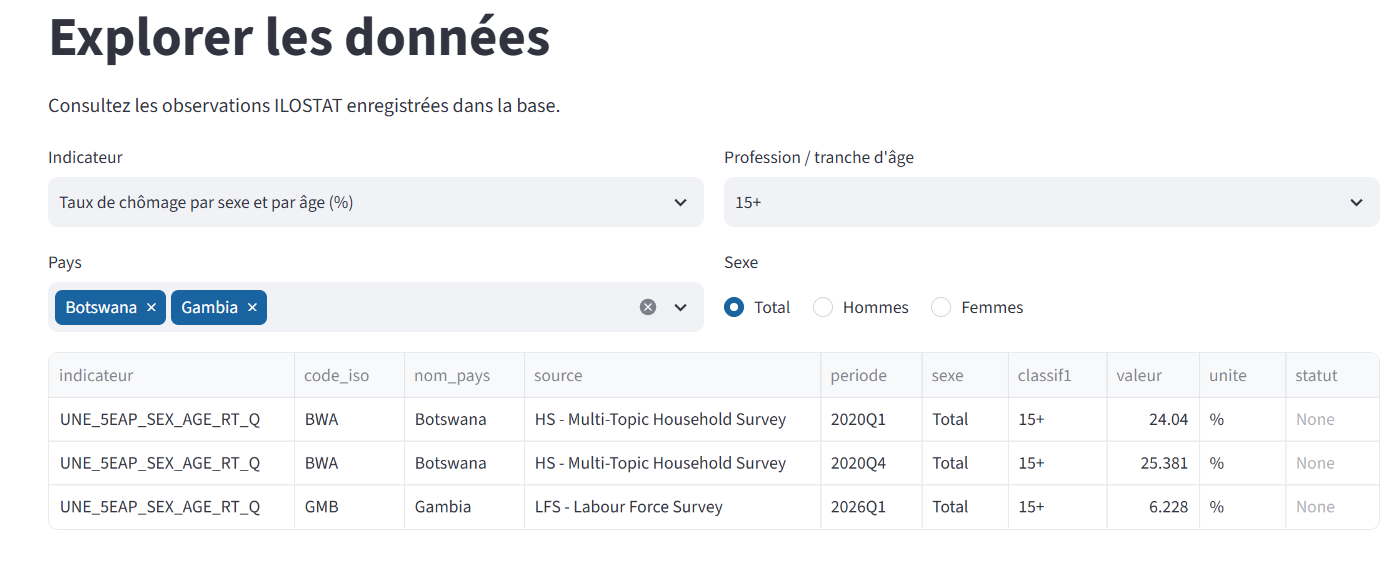
\includegraphics[width=1\linewidth,height=\textheight,keepaspectratio]{images/explorer_tableau.png}

}

\caption{Taux de chômage des 15 ans et plus au Botswana et en Gambie}

\end{figure}%

Le tableau ne contient que trois lignes. Pour le Botswana, on a deux
observations, en 2020Q1 (24,0 \%) et en 2020Q4 (25,4 \%), qui viennent
d'une enquête auprès des ménages (« HS - Multi-Topic Household Survey
»). Environ un actif sur quatre y était donc au chômage en 2020. Pour la
Gambie, on n'a qu'une seule observation, en 2026Q1 (6,2 \%), issue d'une
enquête emploi (« LFS - Labour Force Survey »).

Cet exemple montre l'intérêt de la page : avant de comparer ces deux
pays, on voit tout de suite que leurs données datent d'années très
différentes et viennent de deux types d'enquêtes. Une comparaison
directe entre 25 \% et 6 \% doit donc être faite avec prudence. C'est
aussi pour cette raison que les autres fonctionnalités affichent
toujours la période de chaque pays.

\sectiontitre{Evolution d'un indicateur (F3)}

\subsectiontitre{Présentation de la fonctionnalité}

L'évolution d'un indicateur permet de suivre comment une valeur change
au cours du temps, pour un ou plusieurs pays. L'utilisateur choisit
l'indicateur (par exemple le taux d'emploi), les pays, la modalité (une
tranche d'âge comme 15+, ou une profession selon l'indicateur) et le
sexe (Total, Hommes ou Femmes). Il choisit aussi le nombre de derniers
trimestres à afficher, de 2 à 20 (8 par défaut).

La page affiche trois éléments :

\begin{itemize}
\tightlist
\item
  un graphique en courbes avec une courbe par pays, pour voir la
  tendance de la valeur ;
\item
  un graphique en barres qui montre, pour chaque trimestre, la variation
  par rapport au trimestre précédent ;
\item
  un tableau détaillé avec la valeur, la variation absolue et la
  variation en pourcentage.
\end{itemize}

Deux difficultés ont influencé nos choix. D'une part, la base peut
contenir plusieurs sources pour un même pays et un même trimestre : si
on les gardait toutes, le graphique aurait deux points à la même date.
Nous gardons une seule source par pays et par période (la première par
ordre alphabétique). D'autre part, les pays n'ont pas tous le même
nombre de trimestres disponibles : le nombre demandé est donc appliqué
pays par pays, et un pays qui a moins de données que demandé affiche
simplement tout ce qu'il a. Comme le reste de l'application, cette page
n'est accessible qu'aux utilisateurs connectés.

\subsectiontitre{Fonctionnement technique de la fonctionnalité}

La fonctionnalité suit l'architecture en couches de l'application :

\begin{itemize}
\tightlist
\item
  la couche DAO lit en base les observations de l'indicateur pour les
  pays, la modalité et le sexe demandés. Nous avons réutilisé la classe
  ObservationDAO, qui existait déjà ;
\item
  la couche service (classe EvolutionService) fait les calculs avec
  pandas ;
\item
  la couche controller expose le résultat avec FastAPI sur l'endpoint
  GET /analyses/evolution, réservé aux utilisateurs connectés. Elle
  vérifie les paramètres (par exemple, n\_periodes doit être compris
  entre 1 et 40) et renvoie une erreur 404 si l'indicateur n'existe pas
  ;
\item
  la page Streamlit appelle cet endpoint et trace les graphiques avec
  Plotly Express.
\end{itemize}

Le calcul du service se fait en quatre étapes :

\begin{enumerate}
\def\labelenumi{\arabic{enumi}.}
\tightlist
\item
  on garde une seule source par pays et par période ;
\item
  on trie les observations par pays puis par période (le format « 2024Q4
  » se trie dans l'ordre chronologique) ;
\item
  on calcule les variations pays par pays : la variation absolue est la
  valeur moins celle de la période précédente, et la variation en
  pourcentage est cette différence divisée par la valeur précédente ;
\item
  on ne garde que les N dernières périodes de chaque pays.
\end{enumerate}

L'ordre des étapes 3 et 4 est important. Si on coupait avant de
calculer, la première période conservée n'aurait pas de variation. On
calcule donc les variations sur tout l'historique, puis on garde les N
dernières lignes.

Deux cas particuliers sont traités. La première période de chaque pays
n'a pas de période précédente : ses variations valent « vide » (null
dans le JSON) au lieu d'une valeur inventée. Si la valeur précédente est
égale à 0, le pourcentage n'est pas défini (division par zéro) : il est
aussi laissé vide, car l'infini n'est pas accepté par le format JSON.

Le service est testé avec pytest : la base est remplacée par de petites
données écrites à la main, ce qui permet de vérifier les variations, la
coupe aux N dernières périodes pays par pays, le choix d'une seule
source, le tri chronologique, la division par zéro et le cas où aucune
donnée n'existe. L'endpoint est aussi testé (réponse 200, erreur 404,
erreur 422, résultat vide).

\subsectiontitre{Exemple et interprètation}

\sectiontitre{Comparaison entre pays (F4)}

\subsectiontitre{Présentation de la fonctionnalité}

La comparaison entre pays permet de comparer un indicateur entre
plusieurs pays choisis par l'utilisateur, et de voir rapidement quels
pays ont les valeurs les plus hautes et les plus basses. L'utilisateur
choisit l'indicateur (par exemple le taux d'emploi), les pays, la
modalité (une tranche d'âge comme 15+, ou une profession selon
l'indicateur) et le sexe (Total, Hommes ou Femmes). Il choisit aussi
combien de pays il veut voir dans les « plus hauts » et les « plus bas »
(3 par défaut).

La principale subtilité vient des périodes. Tous les pays ne publient
pas leurs données au même rythme : un pays peut avoir des données
jusqu'en 2026 alors qu'un autre s'arrête en 2024. Par défaut, nous
prenons la dernière période disponible de chaque pays. Ainsi, aucun pays
n'est exclu du classement, mais les pays ne sont pas forcément comparés
à la même date. Pour que l'utilisateur ne soit pas trompé, la période de
chaque pays est toujours affichée, et un message prévient quand les
périodes ne sont pas les mêmes. L'utilisateur peut aussi :

\begin{itemize}
\tightlist
\item
  choisir une période précise dans un menu. Si un pays n'a pas de donnée
  pour cette période, on prend sa dernière période avant celle choisie,
  jamais une donnée plus récente ;
\item
  cocher une case pour utiliser la dernière période commune à tous les
  pays choisis. Tous les pays sont alors comparés à la même date. S'il
  n'existe aucune période commune, la page l'indique.
\end{itemize}

Enfin, une case permet d'activer ou non la mise en couleur des pays les
plus hauts (bleu foncé) et les plus bas (bleu clair). Quand elle est
décochée, toutes les barres sont grises. Comme le reste de
l'application, cette page n'est accessible qu'aux utilisateurs
connectés.

\subsectiontitre{Fonctionnement technique}

La fonctionnalité suit l'architecture en couches de l'application :

\begin{itemize}
\tightlist
\item
  la couche DAO lit en base les observations de l'indicateur pour les
  pays, la modalité et le sexe demandés. Nous avons réutilisé la classe
  ObservationDAO, qui existait déjà ;
\item
  la couche service (classe ComparaisonPaysService) fait les calculs
  avec pandas ;
\item
  la couche controller expose le résultat avec FastAPI sur l'endpoint
  GET /analyses/comparaison-pays. Elle renvoie une erreur 404 si
  l'indicateur n'existe pas ;
\item
  la page Streamlit appelle cet endpoint et trace le graphique avec
  Plotly Express.
\end{itemize}

Le service est testé avec pytest : la base est remplacée par de petites
données écrites à la main, ce qui permet de vérifier le classement, le
choix des périodes et les cas particuliers (aucune donnée, aucune
période commune).

\subsectiontitre{Exemple et interprétation}

On compare le nombre de personnes en emploi (indicateur « Emploi par
sexe et profession », toutes professions confondues, hommes et femmes)
entre la France, l'Allemagne, l'Espagne et l'Italie, avec la dernière
période disponible et un pays dans les « plus hauts » et un dans les «
plus bas ».

\begin{figure}[H]

{\centering 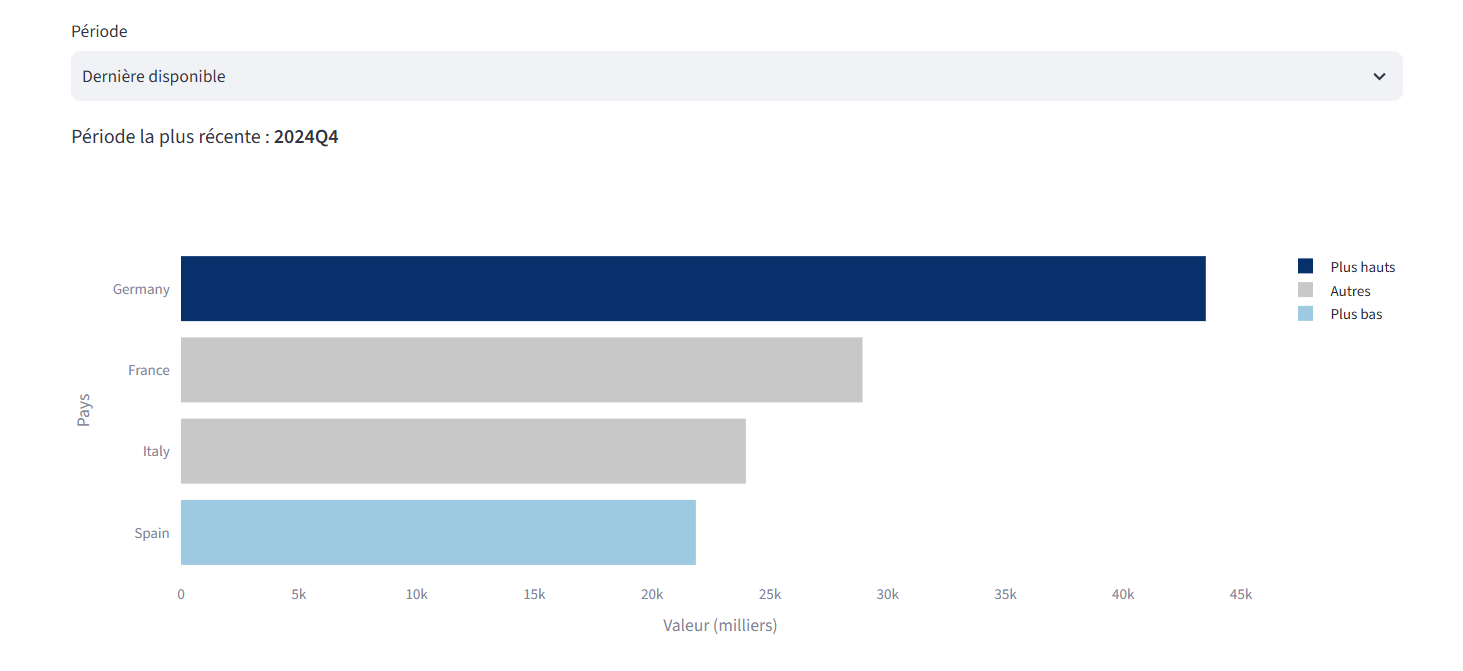
\includegraphics[width=0.95\linewidth,height=\textheight,keepaspectratio]{images/f4_graphique.png}

}

\caption{Nombre de personnes en emploi (en milliers), dernière période
disponible}

\end{figure}%

\begin{figure}[H]

{\centering 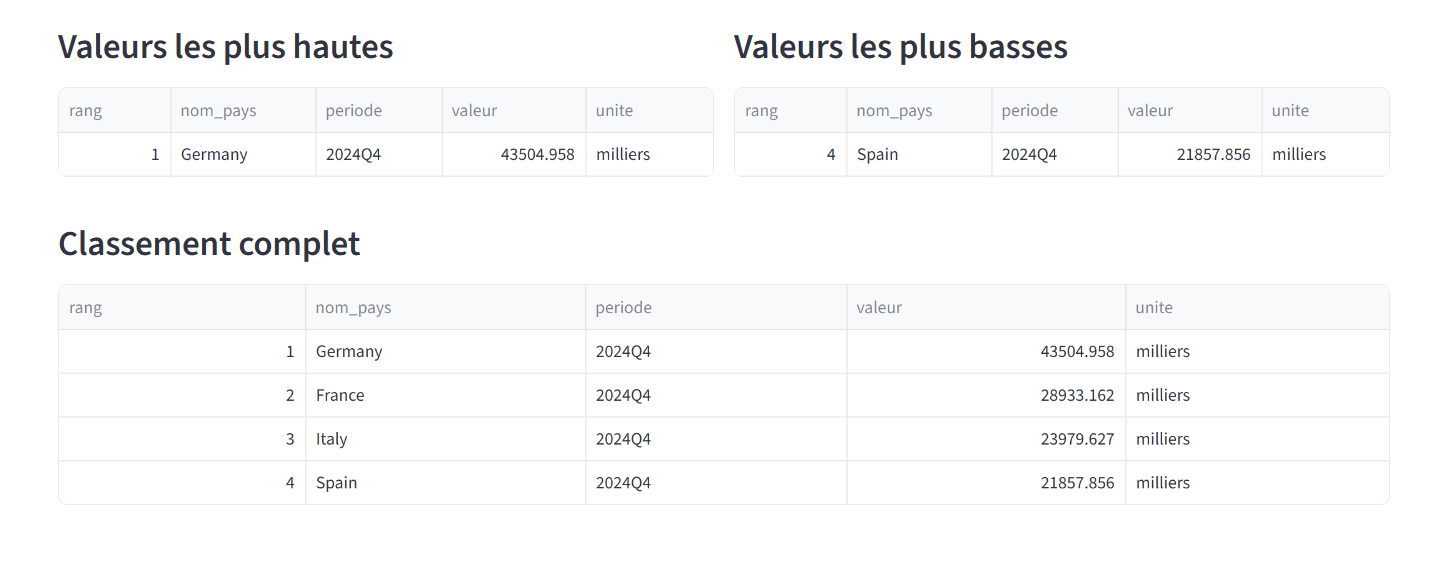
\includegraphics[width=0.95\linewidth,height=\textheight,keepaspectratio]{images/f4_tableaux.png}

}

\caption{Tableaux des valeurs les plus hautes, les plus basses et du
classement complet}

\end{figure}%

Les quatre pays ont tous leur dernière donnée en 2024Q4 : ils sont donc
comparés à la même date et la page n'affiche pas de message
d'avertissement. L'Allemagne arrive en tête avec environ 43,5 millions
de personnes en emploi (en bleu foncé), devant la France (28,9 millions)
et l'Italie (24,0 millions). L'Espagne est en dernière position avec
21,9 millions (en bleu clair), soit à peu près deux fois moins que
l'Allemagne.

Il faut faire attention à l'interprétation : cet indicateur donne un
nombre de personnes et non un taux. Le classement dépend donc beaucoup
de la taille de chaque pays. Pour comparer la situation de l'emploi
entre pays, il est plus pertinent de choisir un indicateur en
pourcentage, comme le taux d'emploi.

\sectiontitre{Carte du monde (FO2)}

\subsectiontitre{Présentation de la fonctionnalité}

La carte du monde affiche un indicateur pour tous les pays de la base,
avec une couleur qui dépend de la valeur : plus la valeur est petite,
plus le bleu est clair, et plus elle est grande, plus il est foncé.
L'utilisateur choisit l'indicateur, la modalité et le sexe, mais pas les
pays, puisque la carte les montre tous. En passant la souris sur un
pays, on voit son nom, sa valeur et la période utilisée. Un tableau sous
la carte reprend toutes les valeurs affichées.

Le choix de la période fonctionne comme pour la comparaison entre pays :
par défaut la dernière période de chaque pays, ou une période choisie
dans un menu, ou la dernière période commune à tous les pays grâce à une
case à cocher. Les pays sans données apparaissent en blanc.

\subsectiontitre{Fonctionnement technique}

La carte réutilise entièrement la fonctionnalité F4. Nous n'avons pas
créé de nouvel endpoint : la page appelle le même endpoint GET
/analyses/comparaison-pays, mais sans préciser de pays, ce qui renvoie
le classement de tous les pays de la base. La carte est tracée avec la
fonction choropleth de Plotly Express. Elle reconnaît directement les
codes ISO à trois lettres des pays (FRA, DEU\ldots), qui sont ceux de
notre base, donc aucun fichier de carte supplémentaire n'a été
nécessaire.

\subsectiontitre{Exemple et interprétation}

On affiche le taux de chômage des 15 ans et plus (hommes et femmes
confondus), avec la dernière période disponible de chaque pays.

\begin{figure}[H]

{\centering 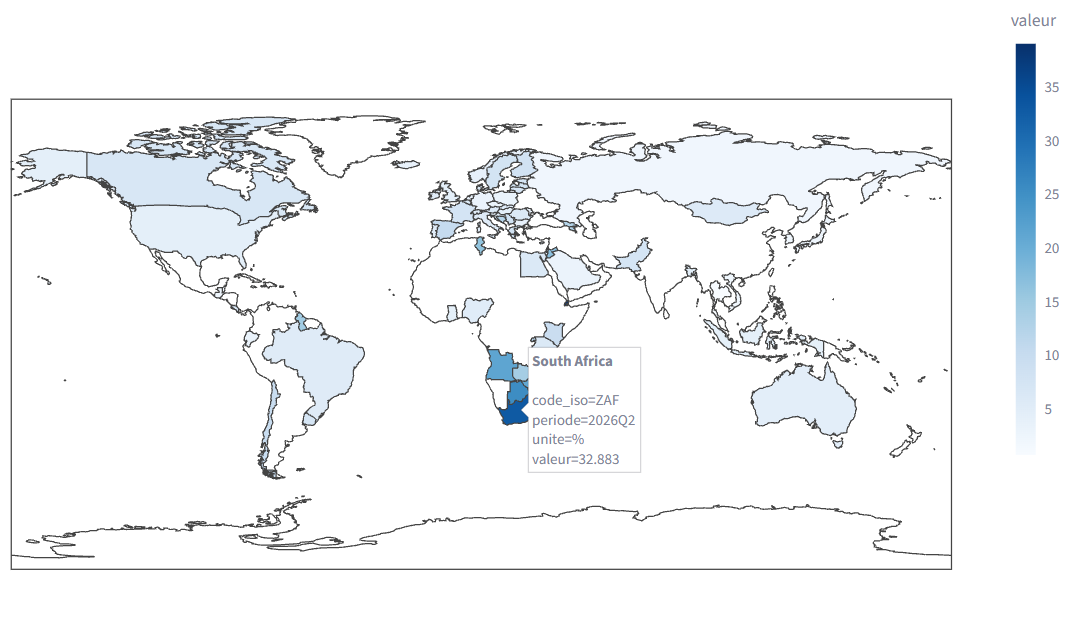
\includegraphics[width=1\linewidth,height=\textheight,keepaspectratio]{images/fo2_carte_chomage.png}

}

\caption{Taux de chômage des 15 ans et plus, dernière période disponible
de chaque pays}

\end{figure}%

La carte montre 79 pays. Sur la capture, la souris est placée sur
l'Afrique du Sud : l'info-bulle indique son taux de chômage (32,9 \%) et
la période utilisée (2026Q2). Les taux les plus élevés sont à Djibouti
(39,0 \%, 2025Q4) et en Afrique du Sud (32,9 \%, 2026Q2), suivis du
Botswana, de l'Angola et du Zimbabwe, tous au-dessus de 20 \%. Les plus
bas sont en Thaïlande (0,7 \%, 2026Q1), au Belize (1,9 \%) et au Viêt
Nam (2,0 \%). La France se situe à 7,5 \% (2024Q4).

Cet exemple montre aussi les limites de la carte. Les 79 pays ne sont
pas comparés à la même date : on trouve 12 périodes différentes, de
2020Q4 pour le Botswana à 2026Q3 pour les plus récentes. La valeur du
Botswana a donc près de six ans d'écart avec celles d'autres pays.
Certains pays n'ont qu'une seule période dans la base, ce qui explique
qu'il n'existe aucune période commune à tous les pays : la case «
dernière période commune » n'est donc utile que pour un petit nombre de
pays. Enfin, seuls les pays importés dans notre base apparaissent en
couleur ; les autres restent en blanc.

\newpage

\sectiontitre{Comparaison multi-indicateurs (F5)}

\subsectiontitre{Présentation de la fonctionnalité}

La comparaison multi-indicateurs permet de superposer jusqu'à quatre
séries sur un même graphique. Elle répond à un besoin fréquent : croiser
des indicateurs qui n'ont ni la même unité ni le même ordre de grandeur,
comme un taux d'emploi (autour de 68 \%), un taux de chômage (autour de
7 à 8 \%) ou un nombre de personnes en emploi (en milliers).

Pour chaque série, l'utilisateur choisit un indicateur, un pays, une
modalité (une tranche d'âge ou une profession selon l'indicateur) et le
sexe. Une case à cocher permet d'activer ou de désactiver chacune des
quatre séries. Chaque série est nommée en langage clair (par exemple «
Taux d'emploi par sexe et âge - FRA - Total - 15+ ») plutôt qu'avec le
code technique d'ILOSTAT. L'utilisateur peut aussi choisir entre deux
affichages :

\begin{itemize}
\tightlist
\item
  l'indice en base 100 : toutes les séries sont ramenées à 100 à une
  même date de départ \(t_0\), ce qui permet de comparer leurs
  évolutions relatives malgré des unités différentes :
\end{itemize}

\[\text{valeur}_{\text{base 100}}(t) = \frac{\text{valeur}(t)}{\text{valeur}(t_0)} \times 100\]

\begin{itemize}
\tightlist
\item
  les valeurs brutes, plus adaptées quand les séries sont dans la même
  unité.
\end{itemize}

Pour que la comparaison reste cohérente, la page applique deux règles.
D'abord, les indicateurs choisis doivent avoir la même fréquence
(trimestrielle ou annuelle) : si on mélange les deux, la page refuse la
comparaison et affiche une erreur. Ensuite, les séries sont alignées sur
leur fenêtre commune : la date de départ est la plus récente des
premières périodes de chaque série. Sous le graphique, un tableau
reprend les données affichées. Comme le reste de l'application, cette
page n'est accessible qu'aux utilisateurs connectés.

\subsectiontitre{Fonctionnement technique}

La fonctionnalité suit l'architecture en couches de l'application :

\begin{itemize}
\tightlist
\item
  le business object \texttt{Selection} regroupe les paramètres d'une
  série (indicateur, pays, modalité, sexe) ;
\item
  la couche DAO récupère les informations de chaque indicateur (libellé,
  unité, fréquence) avec \texttt{IndicateurDAO}, et les observations
  filtrées avec \texttt{ObservationDAO}, qui existait déjà ;
\item
  la couche service (fichier \texttt{multi\_indicateurs\_service.py})
  vérifie que les indicateurs existent et ont la même fréquence,
  supprime les doublons par période, aligne les séries sur la période de
  début commune et calcule la colonne en base 100 avec pandas. Elle
  construit aussi les intitulés lisibles des séries ;
\item
  la couche controller expose le résultat avec FastAPI sur l'endpoint
  POST /analyses/multi-indicateurs. Elle reçoit la liste des séries
  actives et l'option base 100, puis renvoie les séries calculées au
  format JSON ;
\item
  la page Streamlit affiche les quatre colonnes de sélection (les
  modalités proposées dépendent de l'indicateur choisi), met en cache
  les listes d'indicateurs et de pays, et trace le graphique avec Plotly
  Express (infobulles, zoom, légende cliquable).
\end{itemize}

Le service et le controller sont testés avec pytest, et le code est
contrôlé avec ruff.

\subsectiontitre{Exemple et interprétation}

On compare, pour la France, le taux d'emploi (15 ans et plus, hommes et
femmes confondus) et le taux de chômage, de 2020Q1 à 2024Q4, en base
100.

\begin{figure}[H]

{\centering 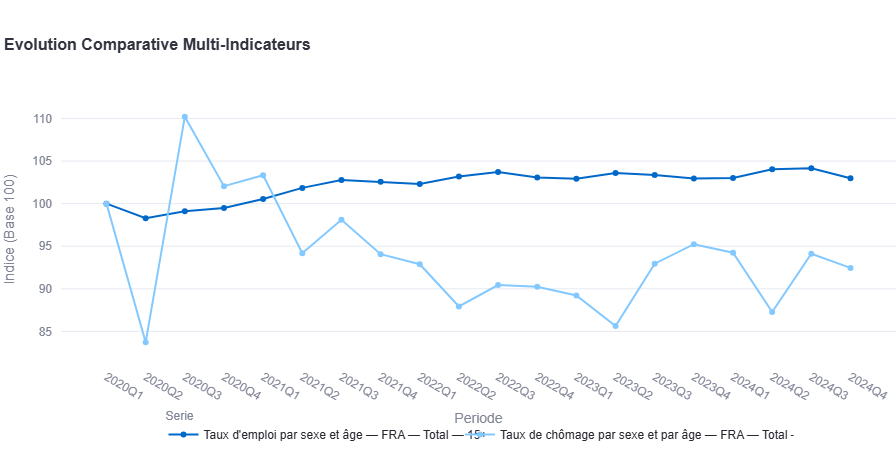
\includegraphics[width=0.92\linewidth,height=\textheight,keepaspectratio]{images/evolution-comparative-multi-indicateurs.png}

}

\caption{Taux d'emploi et taux de chômage de la France en base 100
(2020Q1 à 2024Q4)}

\end{figure}%

Les deux séries démarrent à 100 en 2020Q1, ce qui permet de comparer
leurs variations malgré des niveaux de départ très différents. En
2020Q2, le taux de chômage chute autour de 84, puis remonte à 110,2 en
2020Q3, tandis que le taux d'emploi baisse légèrement à 98,3 en 2020Q2.
Ce mouvement du chômage s'explique en partie par un effet statistique :
pendant le premier confinement, beaucoup de personnes sans emploi ont
cessé de chercher du travail et ont donc été comptées comme inactives. À
partir de 2021Q1, les deux courbes s'écartent : le taux d'emploi se
stabilise entre 103 et 104 (soit 3 à 4 \% de plus qu'au début de 2020),
alors que le taux de chômage reste sous son niveau initial, entre 86 et
95.

Il faut faire attention à la lecture d'un indice en base 100 : il mesure
une variation relative, pas une variation en points de pourcentage. Un
taux de chômage à l'indice 90 signifie que le taux a baissé de 10 \% par
rapport à 2020Q1 (par exemple de 7,5 \% à 6,75 \%), et non de 10 points.
Le résultat dépend aussi de la date de départ : un point de départ
différent changerait l'allure des courbes.

\sectiontitre{Rapport PDF (F03)}

\subsectiontitre{Présentation de la fonctionnalité}

La page « Rapport PDF » permet à l'utilisateur de télécharger un rapport
d'analyse comparative, sans avoir à copier lui-même les graphiques et
les chiffres. Il choisit un indicateur, les pays à comparer et une
période, et l'application génère automatiquement un document PDF de
quatre parties :

\begin{itemize}
\tightlist
\item
  un rappel des paramètres choisis : l'intitulé complet de l'indicateur,
  son unité et son code ILOSTAT entre crochets, ce qui permet de
  retrouver la source ;
\item
  un graphique de l'évolution de l'indicateur pour chaque pays ;
\item
  un tableau de statistiques par pays : minimum, maximum, moyenne et
  variation sur la période ;
\item
  une conclusion rédigée automatiquement à partir de ces statistiques.
\end{itemize}

\subsectiontitre{Fonctionnement technique}

Le graphique du rapport est tracé côté serveur avec Matplotlib en mode
\texttt{Agg}, qui permet de produire une image sans affichage à l'écran.

\subsectiontitre{Exemple et interprétation}

On génère le rapport pour l'indicateur « Emploi par sexe et profession
(milliers) », en comparant l'Allemagne et la France de 2023Q1 à 2024Q4.

\begin{figure}[H]

{\centering 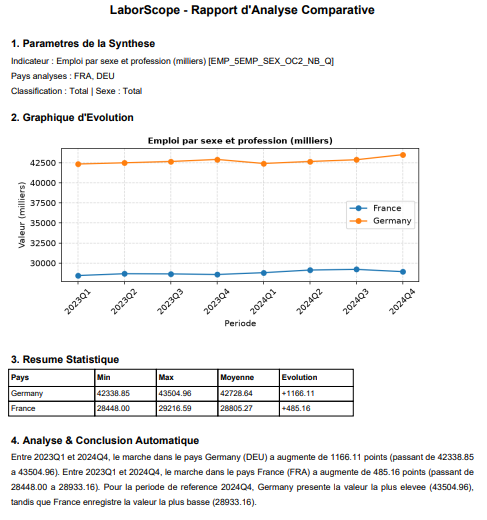
\includegraphics[width=1\linewidth,height=\textheight,keepaspectratio]{images/telechargement.PNG}

}

\caption{Exemple de rapport PDF généré par LaborScope}

\end{figure}%

Le graphique met tout d'abord en évidence un écart de niveau structurel
important entre les deux marchés du travail : sur l'ensemble de la
période étudiée (2023Q1 à 2024Q4), l'emploi total en Allemagne oscille
entre 42 338,85 et 43 504,96 milliers de personnes (soit environ 42,3 à
43,5 millions d'actifs occupés), contre 28 448,00 à 29 216,59 milliers
en France (environ 28,4 à 29,2 millions). Cet écart de près de 14
millions d'emplois s'explique d'abord par la différence de taille
démographique entre les deux pays (environ 84 millions d'habitants en
Allemagne contre 68 millions en France), mais aussi par un taux d'emploi
structurellement plus élevé , notamment chez les seniors et dans le
recours au temps partiel.

Au-delà de ce décalage de volume, l'analyse des variations permet
d'apprécier le dynamisme respectif des créations nettes d'emplois sur la
période : l'emploi total progresse de +1 166,11 milliers en Allemagne
(soit une hausse relative d'environ +2,75 \% entre début 2023 et fin
2024), contre +485,16 milliers en France (soit environ +1,71 \%). Sur
cette fenêtre temporelle, le marché du travail allemand affiche donc un
volume de créations nettes plus de deux fois supérieur à celui de la
France, porté notamment par la croissance des emplois dans le secteur
des services (santé, action sociale, éducation et administration
publique) et par les flux d'immigration active qui soutiennent l'offre
de travail face au vieillissement démographique.\\
L'utilisateur dispose ainsi, en un seul document PDF, des ordres de
grandeur absolus et des amplitudes de variation pour appuyer son
diagnostic économique..

Comme pour la comparaison entre pays (F4), cet indicateur est un nombre
de personnes et non un taux : l'écart entre les deux pays reflète
surtout leur taille, et non la situation de leur marché du travail. Le
rapport est surtout utile pour garder une trace des paramètres et des
chiffres consultés, avec la source de chaque donnée.

\mychapter{Retour sur le projet}

\sectiontitre{Témoignage de Christian}

Une dynamique de groupe bienveillante et structurée

Ces trois mois passés aux côtés de mes camarades à concevoir et
développer l'application LaborScope ont constitué une expérience
particulièrement enrichissante, tant sur le plan humain que technique.
Au-delà de l'aspect purement académique, ce projet a avant tout permis
de tisser une véritable relation amicale au sein du groupe. Travailler
dans un climat de confiance, d'écoute et de bonne humeur avec chacun des
membres de l'équipe a été un moteur essentiel tout au long du semestre.

Au démarrage du projet, lors de sa présentation initiale, j'ai ressenti
une certaine appréhension : j'avais du mal à cerner concrètement
l'ampleur des attentes et la manière dont les différentes briques de
l'application allaient s'articuler entre elles. C'est grâce aux échanges
réguliers lors de nos séances de travail que j'ai progressivement levé
ces zones d'ombre, jusqu'à m'approprier pleinement les objectifs et la
logique globale du projet.

L'organisation mise en place par le groupe a largement contribué à cette
réussite. Le découpage clair du travail étape par étape initié par
Laurent, avec des objectifs précis et des livrables attendus à chaque
jalon, nous a donné un cadre rassurant et efficace pour avancer sans
nous disperser. De son côté, l'appui précieux de Clarence lors des
phases de débogage et de résolution de blocages techniques m'a permis de
surmonter rapidement des situations complexes et de gagner en autonomie.

Une vision d'ensemble grâce au développement des fonctionnalités F5 et
F03

La réalisation de la comparaison multi-indicateurs (F5) et de la
génération de rapport PDF (FO3) a joué un rôle charnière dans ma montée
en compétence. Parce que la fonctionnalité F5 se situe au carrefour de
l'application et mobilise les briques développées en amont par
l'ensemble du groupe (référentiels des pays et des indicateurs,
extraction des séries temporelles, gestion des classifications), je ne
pouvais pas me contenter de coder de manière isolée. Il m'a fallu
comprendre en profondeur le fonctionnement du code de mes camarades afin
d'y raccorder proprement mes traitements et d'adapter mon implémentation
à l'existant.

Le développement de la fonctionnalité FO3, permettant le téléchargement
d'un rapport PDF structuré, a prolongé cette logique en me confrontant à
l'automatisation complète de la restitution d'une analyse : assemblage
des métadonnées lisibles (intitulés complets et unités des indicateurs),
génération de graphiques côté serveur, calcul des indicateurs
statistiques clés (minimum, maximum, moyenne, évolution) et synthèse
automatique des résultats. Cette transversalité m'a offert une
compréhension globale de la construction d'une application informatique,
depuis la base de données jusqu'au livrable exploitable par
l'utilisateur final.

Apports techniques et travail collaboratif

Sur le plan technique, ce projet m'a permis de franchir un cap important
dans ma manière de concevoir, structurer et partager du code au sein
d'une équipe. J'ai notamment acquis des compétences essentielles sur
plusieurs plans :

la maîtrise d'une architecture en couches rigoureuse : j'ai appris à
bien distinguer les responsabilités de chaque composant, en séparant
nettement les objets métiers (business\_object) --- qui modélisent les
concepts fondamentaux du domaine comme une sélection d'analyse --- des
couches d'accès aux données (DAO) et de la logique applicative
(services) ;

l'utilisation quotidienne de Git et GitHub : le travail en équipe sur un
dépôt commun m'a permis de me familiariser concrètement avec le
versionnement du code, la gestion des branches par fonctionnalité, les
fusions (merges), la résolution de conflits et la synchronisation
régulière avec les avancées des autres membres du groupe ;

l'articulation entre backend et frontend : j'ai compris comment relier
proprement une API REST exposée avec FastAPI à une interface interactive
développée sous Streamlit, en veillant à la cohérence des formats
échangés et à la gestion des erreurs ;

les bonnes pratiques de qualité logicielle : l'écriture de tests
unitaires automatisés (pytest) et la vérification systématique du style
de code (ruff) avant chaque partage sur GitHub se sont révélées
indispensables pour sécuriser nos développements collectifs.

En définitive, cette expérience collective m'a permis de consolider
durablement mes compétences en développement logiciel et en travail
collaboratif, tout en me donnant confiance dans ma capacité à mener à
bien un projet informatique complet, de sa conception initiale jusqu'à
son produit final.

\sectiontitre{Témoignage de Clarence}

\sectiontitre{Témoignage d'Antifa}

Dans ce projet, j'ai codé la fonctionnalité d'évolution d'un indicateur
(F3) sur toutes les couches de l'application : le service qui calcule
les variations, l'endpoint, les tests, puis la page Streamlit avec ses
graphiques. J'ai aussi pris en charge une grande partie du dossier :
création du dossier intermédiaire d'analyse, de la page de garde et du
squelette Quarto du dossier final, mise à jour du diagramme
d'architecture avec Christian, rédaction de l'introduction et du
chapitre 1, et mise en forme générale.

Pour être honnête, mon investissement n'a pas été régulier. Au début,
j'ai surtout travaillé sur les documents, alors que le code est arrivé
plus tard, à partir de la semaine 6. Ensuite, certaines semaines n'ont
pas laissé de trace dans nos suivis (charge de travail d'autres
matières, examens, etc). Avec le recul, j'aurais dû commencer la partie
code plus tôt, car F3 s'est retrouvée codée en plusieurs étapes espacées
dans le temps, et le dossier s'est écrit en fin de projet.

Je n'ai jamis été très à l'aise en programmation, et la fiche de tâches
de Laurent m'a été très utile : elle expliquait les étapes, les fichiers
à écrire et les pièges à éviter. Je reconnais que sans elle, j'aurais eu
du mal à avancer seule. Ce qui m'a vraiment fait comprendre
l'application, c'est de suivre le trajet d'une requête, de l'URL jusqu'à
la base de données, puis le retour sous forme de graphique. Les outils
d'IA m'ont beaucoup aidée pour comprendre les erreurs et les pièges de
pandas, comme les valeurs vides ou la division par zéro, mais j'ai dû
vérifier moi-même le résultat avec les tests et avec des exemples.

Les principales difficultés ont été techniques. Git m'a posé beaucoup de
problèmes : push refusé, conflits sur un même fichier, fichiers modifiés
que je ne reconnaissais pas. J'ai aussi eu du mal avec l'organisation
des tests et les imports du backend. Certains de mes commits ont un
message trop vague, et Clarence a dû relire et corriger une partie de
mon code (par exemple la structure du schéma), ce qui est normal pour la
qualité du projet, mais montre que j'ai encore des progrès à faire en
rigueur.

Je retiens que la qualité d'un projet vient autant de l'organisation et
des tests que du code lui-même : détail à première vue anodin, comme
l'ordre entre le calcul des variations et la coupe aux N dernières
périodes, change complètement le résultat affiché. Je retiens aussi que
F3 reste imparfaite : un trimestre manquant n'est pas signalé, et la
variation est alors calculée entre deux observations qui ne sont pas
consécutives.

Si c'était à refaire, je répartirais mon temps de façon plus régulière,
je commencerais le code avant les documents, et je commiterais plus
souvent avec des messages clairs. Cette expérience m'a appris à
travailler en équipe sur un projet de cette taille, et je m'en servirai
pour les futurs projets.

\sectiontitre{Témoignage de Laurent}

\sectiontitre{Témoignage de William}

Dans ce projet, je me suis occupé de la comparaison d'un indicateur
entre pays (F4) et de la carte du monde (FO2). J'ai codé ces deux
fonctionnalités sur toutes les couches de l'application, du service
jusqu'aux pages Streamlit, en passant par l'endpoint et les tests. En
dehors du code, j'ai surtout participé aux réunions, en donnant mon avis
sur la manière dont on voyait le projet et sur ce qu'on voulait faire de
l'application.

Avant le projet, j'étais très faible en programmation. Je pense avoir
beaucoup progressé, en Python mais aussi sur des choses que je n'avais
jamais faites, comme la création d'une API ou d'une interface avec
Streamlit.

Les rôles se sont répartis assez naturellement. Chacun connaissait ses
points forts, et nous n'avons pas eu besoin de désigner un chef de
projet ou un référent technique. On se faisait confiance, on s'écoutait
et on suivait le plan fixé ensemble, ce qui a rendu le travail très
agréable.

Ce plan est pour moi le point fort du projet. Laurent a passé du temps à
préparer, avec l'aide de l'IA, une fiche détaillée pour chaque membre :
les tâches à réaliser, des étapes claires, des indications et des
tutoriels. Chacun pouvait donc avancer de façon autonome et à son
rythme, sans trop dépendre des autres, tout en ayant déjà des aides à
disposition. Je pense que cette organisation nous a rendus efficaces.

J'ai surtout appris comment se construit un projet de cette taille, en
particulier l'architecture technique en couches et l'utilisation des
API. Le moment où j'ai vraiment compris le fonctionnement de l'ensemble,
c'est en suivant le trajet d'une requête, depuis l'URL jusqu'à la base
de données, puis le retour.

Les difficultés ont surtout été techniques, liées à la programmation
elle-même, qui n'est pas mon point fort. Les outils d'IA, conseillés par
l'équipe enseignante pour ce projet, m'ont beaucoup aidé sur ce point :
ils permettent de comprendre un problème très rapidement, ce qui m'a
souvent débloqué.

Ce que je retiens avant tout, c'est la répartition et l'organisation du
travail, qui ont très bien fonctionné. Avec le recul, la seule chose que
je changerais serait de commencer la rédaction du rapport plus tôt. Si
cette façon de travailler est possible en stage ou en entreprise, je la
reprendrai volontiers.

\newpage

\mychapterstar{CONCLUSION}

Le projet \textbf{Laborscope} avait pour objectif de concevoir une
application d'analyse interactive du marché du travail mondial à partir
des données ILOSTAT. Il aboutit à une application fonctionnelle de bout
en bout : une base PostgreSQL alimentée par les données de
l'Organisation internationale du travail, une API REST développée avec
FastAPI, et une interface web (réalisée avec Streamlit) permettant
d'explorer les indicateurs, de les comparer entre pays, de suivre leur
évolution dans le temps ,les visualiser sur une carte du monde et
surtout imprimer les informations voulues en format pdf.

Sur le plan technique, l'architecture en couches (controllers, services,
DAO) et la séparation entre backend et frontend se sont révélées
pertinentes. Elles ont permis de répartir le travail entre les membres
du groupe, de développer en parallèle sans se bloquer mutuellement, et
de tester chaque couche séparément. Les tests automatisés avec pytest,
la gestion de l'environnement avec uv et l'utilisation de Git ont
renforcé la fiabilité et la reproductibilité du projet.

Ce travail nous a aussi appris à traiter des données réelles, qui sont
rarement parfaites. Nous avons dû gérer des sources multiples pour une
même observation, des périodes manquantes ou des valeurs nulles pouvant
rendre un calcul de variation indéfini. Chaque choix de traitement a dû
être justifié et documenté, car il influence directement les résultats
affichés à l'utilisateur.

Le projet présente néanmoins des limites.Les trimestres manquants ne
sont pas signalés dans le calcul des variations, la qualité des
résultats dépend de la couverture inégale des pays dans ILOSTAT, et les
performances n'ont pas été optimisées pour de très gros volumes de
données.

Plusieurs pistes d'amélioration sont envisageables : ajouter des
analyses statistiques plus poussées (tests, régressions, prévisions),
mettre en cache les requêtes les plus fréquentes, signaler explicitement
les périodes manquantes, enrichir l'application avec d'autres sources de
données, et déployer l'ensemble sur un serveur accessible en ligne.

Enfin, ce projet a été une expérience formatrice de travail en équipe :
organisation par fiches de tâches, coordination autour de conventions
communes, relectures croisées et résolution de conflits Git. Il nous a
permis de mettre en pratique, sur un cas concret, les compétences
acquises en programmation, en bases de données et en statistiques durant
notre deuxième année à l'ENSAI.




\end{document}
